\chapter{Sequential CertiKOS Framework}
\label{chap:seq}
In this Chapter, we will provide the formal details
of our sequential \CTOS{} framework.
Section~\ref{sec:seq:layer} introduces
a layer calculus to compose
sequential layers vertically and
horizontally, starting from \emph{layer semantics unit}
(which is language dependent).
This layer calculus is general enough,
such that it is not bounded to any specific language,
and the components of layer interfaces
and types of primitives are treated as parameters. 
In Section~\ref{sec:seq:sound},
we show the proof structure for the soundness of layer calculus.
Section~\ref{sec:seq:clight}
and Section~\ref{sec:seq:lasm}
show how to construct layer semantics unit
and apply layer calculus
in ClightX (\ie, a C-like language) and LAsm (\ie, an assembly language), respectively.
In Section~\ref{sec:seq:comp},
we introduce CompCertX (\ie, a verified C compiler)
to compile ClightX layers down to assembly-level,
and show how to link the result layers with
LAsm layers.

\section{A Calculus of Sequential Abstraction Layers}
\label{sec:seq:layer}

\paragraph{Motivation}

A user of an abstraction layer $\layer{L_1}{M}{L_2}$ wants to know
that its implementation $M$ (on top of the underlay interface $L_1$)
can be used to run any program $P$ written against the overlay
interface $L_2$.
If we consider $L_1, L_2$ as abstract machines
and $M$ as a program transformation (which transforms
a program $P$ into $M(P)$), 
then for some notion of refinement $\sqsubseteq$,
this property can be stated as
$\forall P \,.\, M(P) @ L_1 \sqsubseteq P @ L_2$,
meaning that the behavior of $M(P)$ executing
on top of the underlay specification $L_1$
refines that of the program $P$
executing on top of the overlay specification $L_2$.

This view of abstraction layers captures a wide variety of situations.
Furthermore, two layers $\layer{L_1}{M}{L_2}$ and
$\layer{L_2}{N}{L_3}$ can be composed as $\layer{L_1}{M \circ
  N}{L_3}$, and the correctness of the layer implementation $M \circ
N$ follows from that of $M$ and $N$.  
%This gives us a way to decompose
%layer implementations into a succession of smaller and
%easier-to-verify components.

However, 
% this paradigm is ill-suited for implementation purposes.
% An unrestricted program transformation is often too
% general to describe what is actually going on: 
the layer interfaces
are often not arbitrary abstract machines, but simply instances of a base
language, specialized to provide layer-specific primitives and
abstract state.  The implementation is not an arbitrary
transformation, but instead consists of some library code to be linked
with the client program.  In order to prove this transformation correct,
we will verify the implementation of each primitive
separately, and then use these proofs in conjunction with a
general template for the instrumented language.

Abstract machines and program transformations are too general to
capture this redundant structure.  The sequential layer calculus
presented in this section provides fine-grained notions of layer
interfaces and implementations.  It allows us to describe what varies
from one layer to the next and to assemble such layers 
%from their components 
in a generic way.

\subsection{Prerequisites}

To keep the formalism general and simple,
we initially take the syntax and behavior of the programs
under consideration to be abstract parameters.
Specifically,
in the remainder of this section we will assume that
the following are given:
\begin{itemize}
\item a set of identifiers $i \in \integer$
    which will be used to name variables, functions, and primitives
    (\eg, \textsf{deQ} and \textsf{tcbp} in Figure~\ref{fig:queue});
\item sets of function definitions $\kappa \in \mathbb{K}$ and
    variable definitions $\nu \in \mathbb{T}$,
    as specified by the language
    (\eg, $\kappa_\textsf{deQ}$ and $\nu_\textsf{tcbp}$ in Figure~\ref{fig:queue});
% XXX: identifiers?
\item a set of behaviors $\sigma \in \Sigma$
    for the individual primitives of layers
    and the individual functions of programs
    (\eg, the step relation $\sigma_\textsf{deQ}$ 
    	derived from the Coq function 
    	$\spec_\textsf{deQ}$ in Figure~\ref{fig:queue}).
\end{itemize}
For example, in the model given in Section~\ref{sec:seq:clight},
we will use step relations as the behaviors.
Function definitions will include the functions' formal parameters and bodies
(but not their names),
whereas definitions of variables
will specify their types and initialization data.
% XXX: but for now completely abstract

We also need to define how the behaviors
refine one another.
This is particularly important because
our layer interfaces bundle primitive specifications,
and because a relation between layer interfaces is defined pointwise
over these primitives. Ultimately, we wish to use these
fine-grained layers and refinements to build complete abstract
machines and whole-machine simulations. 
%FIXME: improve:
%Yet, ultimately we wish to use these
%fine-grained layers and refinements
%to build complete abstract machines and whole-machine simulations.
This can only be done
if the refinements of individual primitives are consistent;
for example, if they are given in terms of the same simulation relation.

Hence, we index behavior refinement by
the elements of a partial monoid $(\mathbb{R}, \circ, \id)$.
We will refer to the elements $R \in \mathbb{R}$ of this monoid
as \emph{simulation relations}.
However, note that at this stage,
the elements of $\mathbb{R}$ are entirely abstract,
and we require only that the composition operator $\circ$
and identity element $\id$ satisfy the monoid laws
$R_1 \circ (R_2 \circ R_3) = (R_1 \circ R_2) \circ R_3$ and
$R \circ \id = \id \circ R = R$.

Finally,
we need to interpret these abstract simulation relations
as refinement relations between behaviors.
That is,
for each $R \in \mathbb{R}$, we require
a relation $\lpath{R}$ on $\Sigma$.
For instance,
if the behaviors $\sigma_1, \sigma_2 \in \Sigma$
are taken to be step relations over some sets of states,
$\sigma_1 \le_R \sigma_2$ may be interpreted
as the following simulation diagram:
\[ 
    \xymatrix{
        s_1 \ar[rr]^{\sigma_1} \ar@{-}[d]_R & & s'_1 \ar@{.}[d]^R \\
        s_2 \ar@{.>}[rr]_{\sigma_2} & & s'_2
    }
\]
That is, whenever two states $s_1, s_2$
are related by $R$ in some sense,
and $\sigma_1$ takes $s_1$ to $s_1'$ in one step, then
there exists $s_2'$ such that 
$\sigma_2$ takes $s_2$ to $s_2'$ in zero or more steps,
and $s_2'$ and $s_1'$ are also related by $R$.
The relations $\le_-$ should respect the monoid structure of $\mathbb{R}$,
so that for any $\sigma \in \Sigma$ we have $\sigma \lpath{\id} \sigma$,
and so that whenever $R, S \in \mathbb{R}$
and $\sigma_1, \sigma_2, \sigma_3 \in \Sigma$
such that $\sigma_1 \lpath{R} \sigma_2$ and $\sigma_2 \lpath{S} \sigma_3$,
it should be the case that $\sigma_1 \lpath{S \circ R} \sigma_3$.
% XXX: Possibly summarize laws in a figure instead?

\subsection{Sequential layer interfaces and modules}
\begin{figure}[t]
    \begin{align*}
        \lfloor L \rfloor \in \mathbb{L} &=
            \mathbb{I} \rightharpoonup (\Sigma + \mathrm{T}) &
        \lfloor M \rfloor \in \mathbb{M} &=
            \mathbb{I} \rightharpoonup (\mathrm{K} + \mathrm{T}) \\
        %
        \lfloor \varnothing \rfloor &=
            \bot &
        \lfloor \varnothing \rfloor &=
            \bot \\
        %
        \lfloor i \mapsto \sigma \rfloor &=
            i \mapsto \iota_1(\sigma) &
        \lfloor i \mapsto \kappa \rfloor &=
            i \mapsto \iota_1(\kappa) \\
        %
        \lfloor i \mapsto \nu \rfloor &=
            i \mapsto \iota_2(\nu) &
        \lfloor i \mapsto \nu \rfloor &=
            i \mapsto \iota_2(\nu) \\
        %
        \lfloor L_1 \oplus L_2 \rfloor &=
            \lfloor L_1 \rfloor \cup \lfloor L_2 \rfloor &
        \lfloor M_1 \oplus M_2 \rfloor &=
            \lfloor M_1 \rfloor \cup \lfloor M_2 \rfloor \\
        \lfloor L_1 \lpath{R} L_2 \rfloor &\!\Leftrightarrow
            \lfloor L_1 \rfloor \lpath{R} \lfloor L_2 \rfloor &
        \lfloor M_1 \subseteq M_2 \rfloor &\!\Leftrightarrow
            \lfloor M_1 \rfloor \sqsubseteq \lfloor M_2 \rfloor
    \end{align*}
    \begin{center}
    Where $\lfloor L_1 \rfloor \lpath{R} \lfloor L_2 \rfloor$ means that for all $i \in \mathbb{I}$:
    \begin{align*}
        \forall \sigma_1 \, . \quad
            \lfloor L_1 \rfloor (i) &= \iota_1(\sigma_1) &\Rightarrow\quad
        \exists \sigma_2 \, . \,
            \lfloor L_2 \rfloor (i) &= \iota_1(\sigma_2) \wedge
            \sigma_1 \lpath{R} \sigma_2 \\
        \forall \nu \, . \quad
             \lfloor L_1 \rfloor (i) &= \iota_2(\nu) &\Rightarrow\quad
             \lfloor L_2 \rfloor (i) &= \iota_2(\nu),
    \end{align*}
    and both orders hold when the right-hand side is undefined.
    \end{center}
    \caption{Interpretation of layers and modules as finite maps}
    \label{fig:fmap-layers}
\hrulefill
    \afterpage{\FloatBarrier}
\end{figure}

The syntax of the calculus is defined as follows:
\[\begin{array}{rl}
    L &::= \varnothing
            \ |\ i \mapsto \sigma
            \ |\ i \mapsto \nu
            \ |\ L_1 \oplus L_2 \\
    M &::= \varnothing
            \ |\ i \mapsto \kappa
            \ |\ i \mapsto \nu
            \ |\ M_1 \oplus M_2
\end{array}\]
\noindent{}The layer interfaces $L$ and modules $M$
are essentially finite maps;
constructions of the form $i \mapsto \_$
are elementary single-binding objects,
and $\oplus$ computes
the union of two layers or modules.
This is illustrated by the proof-of-concept
interpretation given in 
Figure~\ref{fig:fmap-layers}.
For example, the sequential thread queue module, shown in Figure~\ref{fig:queue},
can be defined as 
$M_\textsf{thread\_queue}:=\textsf{tcbp}\mapsto \nu_\textsf{tcbp} 
\oplus \textsf{tdqp}\mapsto \nu_\textsf{tdqp}
\oplus \textsf{deQ}\mapsto \kappa_\textsf{deQ}$,
while the overlay interface can be defined as 
$L_\textsf{thread\_queue}:= \textsf{deQ}\mapsto \sigma_\textsf{deQ}$ .

\begin{figure} [t]
    \noindent
    \fbox{$M_1 \subseteq M_2$}
    \vspace*{-17pt}
    \begin{align*}
        M &\subseteq M &
            \rulename{MLe-Refl} \\
        \varnothing &\subseteq M &
            \rulename{MLe-Empty} \\
        M \oplus \varnothing &\subseteq M &
            \rulename{MLe-Id-Right} \\
        (M_1 \oplus M_2) \oplus M_3 &\subseteq M_1 \oplus (M_2 \oplus M_3) &
            \rulename{MLe-Assoc} \\
        M_2 \oplus M_1 &\subseteq M_1 \oplus M_2 &
            \rulename{MLe-Comm} \\
        M_1 &\subseteq M_1 \oplus M_2 &
            \rulename{MLe-Ub-Left} \\
        M_1 \subseteq M_2 \wedge M_2 \subseteq M_3
            &\Rightarrow M_1 \subseteq M_3 &
            \rulename{MLe-Trans} \\
        M_1 \subseteq M_1' \wedge M_2 \subseteq M_2'
            &\Rightarrow M_1 \oplus M_2 \subseteq M_1' \oplus M_2'
            &\rulename{MLe-Mon}
    \end{align*}

    \vspace{1em}
    \noindent
    \fbox{$L_1 \lpath{R} L_2$}
    \vspace*{-17pt}
    \begin{align*}
        L &\lpath{\id} L &
            \rulename{LLe-Refl} \\
        \varnothing &\lpath{R} L &
            \rulename{LLe-Empty} \\
        L \oplus \varnothing &\lpath{\id} L &
            \rulename{LLe-Id-Right} \\
        (L_1 \oplus L_2) \oplus L_3 &\lpath{\id} L_1 \oplus (L_2 \oplus L_3) &
            \rulename{LLe-Assoc} \\
        L_2 \oplus L_1 &\lpath{\id} L_1 \oplus L_2 &
            \rulename{LLe-Comm} \\
        L_1 &\lpath{\id} L_1 \oplus L_2 &
            \rulename{LLe-Ub-Left} \\
        L \oplus L &\lpath{\id} L &
            \rulename{LLe-Idempotent} \\
        L_1 \lpath{R} L_2 \wedge L_2 \lpath{S} L_3 &\,\Rightarrow\,
            L_1 \lpath{S \circ R} L_3 &
            \rulename{LLe-Trans} \\
        L_1 \lpath{R} L_1' \wedge L_2 \lpath{R} L_2' &\,\Rightarrow\,
            L_1 \oplus L_2 \lpath{R} L_1' \oplus L_2' \hspace{-2em} &
            \rulename{LLe-Mon} \\
        \sigma_1 \lpath{R} \sigma_2 &\,\Rightarrow\,
            i \mapsto \sigma_1 \lpath{R} i \mapsto \sigma_2 &
            \rulename{LLe-Intro-Prim}
    \end{align*}

    \vspace{1em}
    \noindent
    \fbox{$\ltyp{L_1}{R}{M}{L_2}$}
    \vspace*{-17pt}
    \begin{prooftree}
        \AxiomC{}
	\RightLabel{\rulename{Empty}}
 	\UnaryInfC{$\ltyp{L}{\id}{\varnothing}{L}$}
    \end{prooftree}
    \begin{prooftree}
        \AxiomC{}
        \RightLabel{\rulename{Var}}
        \UnaryInfC{$\ltyp{L}{\id}{i \mapsto \nu}{i \mapsto \nu}$}
    \end{prooftree}
    \begin{prooftree}
        \AxiomC{$\ltyp{L_1}{R}{M}{L_2}$}
        \AxiomC{$\ltyp{L_2}{S}{N}{L_3}$}
        \RightLabel{\rulename{Vcomp}}
        \BinaryInfC{$\ltyp{L_1}{R \circ S}{M \oplus N}{L_3}$}
    \end{prooftree}
    \begin{prooftree}
        \AxiomC{$\ltyp{L}{R}{M}{L_1}$}
        \AxiomC{$\ltyp{L}{R}{N}{L_2}$}
        \RightLabel{\rulename{Hcomp}}
        \BinaryInfC{$\ltyp{L}{R}{M \oplus N}{L_1 \oplus L_2}$}
    \end{prooftree}
    \begin{prooftree}
        \AxiomC{$L_1 \lpath{R} L_1'$}
        \AxiomC{$\ltyp{L_1}{S}{M}{L_2}$}
        \AxiomC{$L_2' \lpath{T} L_2$}
        \RightLabel{\rulename{Conseq}}
        \TrinaryInfC{$\ltyp{L_1'}{R \circ S \circ T}{M}{L_2'}$}
    \end{prooftree}
    \caption{The fine-grained layer calculus}
    \label{fig:llang}
\hrulefill
    \afterpage{\FloatBarrier}
\end{figure}

The rules are presented in Figure~\ref{fig:llang}.
The inclusion preorder defined on modules
corresponds to the intuition that when $M \subseteq N$,
any definition present in $M$ must be present in $N$ as well.
The composition operator $\oplus$
behaves like a join operator.
However, while $M \oplus N$ is an upper bound of $M$ and $N$,
we do not require it to be the \emph{least} upper bound.
The order on layer interfaces
extends the underlying simulation preorder $\lpath{R}$ on behaviors.
Compared to $\subseteq$, it should satisfy
the additional property \rulename{LLe-Idempotent}.

The judgment $\ltyp{L_1}{R}{M}{L_2}$ is akin to a typing judgment for
modules. It asserts that, using the simulation relation $R$, the
module $M$---running on top of $L_1$---faithfully implements $L_2$.
Because modules consist of code ultimately intended to be linked
with a client program, the empty module $\varnothing$ acts as a
unit and can implement any layer interface $L$ 
(\rulename{Empty}).  Moreover, appending first $N$ then $M$ to a
client program is akin to appending $M \oplus N$ in one step
(\rulename{Vcomp}).  These rules correspond to the identity and
composition properties already present in the framework of abstract
machines and program transformations.  However, the fine-grained
calculus also provides a way to split refinements (\rulename{Hcomp}):
when two different layer interfaces are implemented \emph{in a
  compatible way} by two different modules on top of a common underlay
interface, then the union of the two modules implements the union of
the two interfaces.

This allows us to break down the problem of verifying a layer
implementation in smaller pieces, but ultimately, we need to handle
individual functions and primitives.  The consequence rule
(\rulename{Conseq}) can be used to tie our notion of behavior
refinement into the calculus.  However, to make the introduction of
certified code possible, we need a semantics of the underlying
language.

\subsection{Language semantics}
\label{ssec:layer-langsem}

\begin{figure}[t]
\begin{align*}%
\llbracket - \rrbracket &\ \,:\ \,\mathbb{M} \rightarrow (\mathbb{L} \rightarrow \mathbb{L}) \\
        i \mapsto \nu &\lpath{\id}
            \llbracket i \mapsto \nu \rrbracket L &
            \rulename{Sem-Var} \\
        \llbracket M \rrbracket (L \oplus \llbracket N \rrbracket L)
            &\lpath{\id}
            \llbracket M \oplus N \rrbracket L &
            \rulename{Sem-Comp} \\
        M_1 \subseteq M_2 \wedge L_1 \lpath{R} L_2 &\,\Rightarrow\,
            \llbracket M_1 \rrbracket L_1 \lpath{R}
            \llbracket M_2 \rrbracket L_2 &
            \rulename{Sem-Mon}%
\end{align*}
\caption{Semantics of modules}
\label{fig:msem}
\hrulefill
    \afterpage{\FloatBarrier}
\end{figure}

Assume that layers and modules are interpreted in the respective sets
$\mathbb{L}$ and $\mathbb{M}$.  The semantics of a module can be
understood as the effect  its code has on the underlay
interface, as specified by a function $\llbracket - \rrbracket :
\mathbb{M} \rightarrow \mathbb{L} \rightarrow \mathbb{L}$.  Given such
a function, we can interpret the typing judgment as:
\[ \ltyp{L_1}{R}{M}{L_2} \quad \Leftrightarrow \quad
   L_2 \lpath{R} L_1 \oplus \llbracket M \rrbracket L_1. \]
\noindent{}Then the properties in Figure~\ref{fig:msem}
are sufficient to ensure the soundness of the typing rules
with respect to this interpretation.

Here, surprisingly, we require that the specification refine the
implementation!  This is because our proof technique involves turning
such a \emph{downward} simulation into the converse \emph{upward}
simulation, as detailed in Section~\ref{sec:seq:lasm}
(Theorem~\ref{thm:sound}) and Section~\ref{sec:clightx-prog}.  Also, we
included $L_1$ on the right-hand side of $\lpath{R}$ to support
pass-through of primitives in the underlay $L_1$ into the overlay
$L_2$.

The property \rulename{Sem-Comp} can be understood intuitively as
follows.  In $\llbracket M \rrbracket (L \oplus \llbracket N
\rrbracket L)$, the code of $M$ is able to use the functions defined
in $N$ in addition to the primitives of the underlay interface $L$,
but conversely the code of $N$ cannot access the functions of $M$.
However, in $\llbracket M \oplus N \rrbracket L$, the functions of $M$
and $N$ can call each other freely, and therefore the result should be
more defined.  The property \rulename{Sem-Mon} states that making the
module and underlay larger should also result in a more defined
semantics.

Once a language semantics is given, we introduce a
language-specific rule to prove the correctness of individual functions: 
    \AxiomC{$\text{VC}(L, \kappa, \sigma)$}
    \RightLabel{\rulename{Fun}}
    \UnaryInfC{$\ltyp{L}{\id}{i \mapsto \kappa}{i \mapsto \sigma}$}
    \[ \DisplayProof \]
%\end{prooftree}
The \emph{semantics layer unit} $\text{VC}(L, \kappa, \sigma)$
is a language-specific predicate, 
which asserts that the function body $\kappa$ faithfully implements the
primitive behavior $\sigma$ on top of $L$.  
This rule can be combined with the rules of the calculus to build up
complete certified layer implementations.

Similarly, given a concrete language semantics, we will want to tie
the calculus back into the framework of abstract machines and program
transformations.  
The \emph{abstract machine}
we use is defined as below:
\begin{definition}[Abstract Machine]
\label{def:mach}
An \emph{abstract machine} is a tuple $\Mach = (\statet, \rightarrow, I, F)$
where $\statet$ is a set of states,
$\rightarrow \, \subseteq \statet \times \statet$ is a transition relation,
$I \subseteq \statet$ is a set of initial states, and
$F \subseteq \statet$ is a set of final states.
\end{definition}

\ignore{
\begin{definition}[Safety]
Given a machine $\Mach$,
we say that $s \in S$ is a \emph{stuck state}
if $s \notin F$ and there is no $s'$ such that $s \rightarrow s'$.
Then, a \emph{safe state} is a state $s$ such that there is no
stuck state $s'$ with $s \rightarrow^* s'$.
%A \emph{safe machine} is a machine which has at least one initial state,
%and for which all initial states are safe.
\end{definition}
}

\noindent{}Thus, for a layer interface $L$, we define a
corresponding abstract machine 
\[P@L:= (\statet(L), 
\stackrel{L}{\rightarrow}, I(P), F)\]
, which means to execute program $P$ written in a
version of the language augmented with the primitives specified in
$L$. 
 The program transformation associated with a module $M$ will
simply concatenate the code of $M$ to the client program.  Then, for a
particular notion of refinement $\sqsubseteq$, we will want to prove
that the typing judgments entail the contextual refinement property:
%\begin{prooftree}
    \AxiomC{$\ltyp{L_1}{R}{M}{L_2}$}
    %\RightLabel{\rulename{xxx}}
    \UnaryInfC{$\forall P \,.\,
        (P \oplus M)@L_1 \sqsubseteq P@L_2$}
    \[ \DisplayProof \]
%\end{prooftree}

\noindent{}Informally, if $M$ faithfully implements $L_2$ on top of
$L_1$, then invocations in $P$ of a primitive $i$ with behavior
$\sigma$ in $L_2$ can be satisfied by calling the corresponding
function $\kappa$ in $M$.

Indeed in Section~\ref{sec:seq:clight} and Section~\ref{sec:seq:lasm}, the primitive
specifications in $\llbracket M \rrbracket L$, based on step
relations, are defined to reflect the possible executions of the
function definitions in $M$.  Therefore, $L_2 \le_R L_1 \oplus
\llbracket M \rrbracket L_1$ implies that, for any primitive
implementation in $M$, the corresponding deep specification in $L_2$
refines the execution of that function definition.  Hence the
execution of program $P$ with underlay $L_2$ refines that of $P \oplus
M$ with underlay $L_1$ (the properties enumerated in
Figure~\ref{fig:msem} hold for a similar reason).  Properties of the
language (\ie, being determinate and receptive) can then be used to
reverse this refinement into the desired $(P \oplus M)@L_1 \sqsubseteq
P@L_2$.


\section{Soundness of Layer Calculus}
\label{sec:seq:sound}
The \emph{soundness} of the layer calculus 
can be proved by case analysis over all the rules.
First,
    under our interpretation of the typing judgment,
    \rulename{Empty} corresponds directly to \rulename{LLe-Ub-Left}.
    In fact, the judgment $\ltyp{L}{\id}{M}{L}$
    holds for any module $M$.

The soundness of \rulename{Conseq} is
    straightforward to establish as well:
    by the monotonicity of  $\oplus$ and $\llbracket - \rrbracket$,
    $L_1 \lpath{R} L_1'$ entails:
    \[ L_1  \oplus \llbracket M \rrbracket L_1 \lpath{R}
       L_1' \oplus \llbracket M \rrbracket L_1' \]
    , which combined with the other premises gives us:
    \[ L_2' \lpath{T} L_2 \lpath{S}
       L_1  \oplus \llbracket M \rrbracket L_1 \lpath{R}
       L_1' \oplus \llbracket M \rrbracket L_1' \]
    Hence, by \rulename{LLe-Trans}:
    \[ L_2' \lpath{R \circ S \circ T} L_1' \oplus \llbracket M \rrbracket L_1' \]

The property \rulename{Sem-Comp} can be used to prove
    the soundness of \rulename{Vcomp}.
    If $L_3 \lpath{S} L_2 \oplus \llbracket N \rrbracket L_2$ and
    $L_2 \lpath{R} L_1 \oplus \llbracket N \rrbracket L_1$,
    then by monotonicity we get:
    \[ L_3 \lpath{R \circ S} L_1 \oplus \llbracket N \rrbracket L_1 \oplus
      \llbracket M \rrbracket (L_1 \oplus \llbracket N \rrbracket L_1) \]
    Applying \rulename{Sem-Comp}
    on the right-hand side of $\oplus$, we get:
    \[ L_3 \lpath{R \circ S} L_1 \oplus \llbracket N \rrbracket L_1
                           \oplus \llbracket M \oplus N \rrbracket L_1 \]
    This can be further rewritten by exploiting the fact that
    $\llbracket N \rrbracket L_1 \lpath{\id}
     \llbracket M \oplus N \rrbracket L_1$
    together with \rulename{LLe-Idempotent},
    which allows us to conclude:
    \[ L_3 \lpath{R \circ S} L_1 \oplus \llbracket M \oplus N \rrbracket L_1 \]

Finally, the soundness of \rulename{Hcomp} can be demonstrated as follows.
    If we know that $L_1 \lpath{R} L \oplus \llbracket M \rrbracket L$
    and that $L_2 \lpath{R} L \oplus \llbracket N \rrbracket L$,
    then by the monotonicity of $\oplus$:
    \[ L_1 \oplus L_2 \lpath{R} (L \oplus \llbracket N \rrbracket L)
                         \oplus (L \oplus \llbracket M \rrbracket L). \]
    Since $M \lpath{\id} M \oplus N$
    and $N \lpath{\id} M \oplus N$,
    this can be further rearranged as:
    \[ L_1 \oplus L_2 \lpath{R} (L \oplus L) \oplus
        (\llbracket M \oplus N \rrbracket L \oplus
         \llbracket M \oplus N \rrbracket L). \]
    We can conclude using \rulename{LLe-Idempotent}:
    \[ L_1 \oplus L_2 \lpath{R} L \oplus \llbracket M \oplus N \rrbracket L. \]
% FIXME: uniform notation?

%\subsection{Deriving abstract machines and simulations}
%
%[Even though we remain totally abstract in this section,
%probably we can already give an idea of what's involved,
%independent of the actual language used.]
\section{Layered programming in ClightX}
\label{sec:seq:clight}

In this section, we provide an instantiation of our framework for a
C-like language. This instantiation serves two purposes: it
illustrates a common use case for our framework, showing its usability
and practicality; and it shows that our framework can add
modularization and proof infrastructure to existing language subsets
at minimal cost.

\paragraph{Our starting point: CompCert Clight}

Clight~\cite{blazy-leroy-clight} is a subset of C and is
formalized in Coq as part of the CompCert project.  Its formal
semantics relies on a memory model~\cite{leroy08} that is not only
realistic enough to specify C pointer operations, but also designed to
simplify reasoning about non-aliasing of different
variables (making sense of the standard notion of C ``object'').
From the programmer's point of view, 
Clight avoids most pitfalls and peculiarities of C such
as nondeterminism in expressions with side effects. 
On the other hand,
Clight allows for pointer arithmetic and is a true subset of C: valid
Clight programs are valid C programs with the same semantics.
Such
simplicity and practicality turn Clight into a solid choice for
certified programming.
Furthermore,
the CompCert verified compiler
provides strong guarantees on code
obtained by compilation of Clight programs.
However, Clight provides little support for abstraction,
and proving properties
about a Clight program requires intricate reasoning about
data structures. This issue is addressed by our layer infrastructure.


In this section, we first describe how to instrument the CompCert
languages with abstract state and primitives. Then, we describe the
syntax and semantics of the ClightX language. Finally, we show
examples of layered programming and verification using the abstract
state and primitives.

\subsection{Abstract state, primitives, and layer interfaces}

We enable abstraction in Clight and other CompCert languages
by instrumenting the memory states used by their semantics
with an \emph{abstract state} component.
This abstract state can be manipulated using \emph{primitives},
which are made available through CompCert's external function mechanism.
We call the resulting language ClightX.

%\vspace*{-3pt}
\paragraph{Abstract state and external functions}
The abstract state is not just a ghost state for reasoning: it
does influence the outcome of executions!  However, we seek to
minimize its impact on the existing proof
infrastructure for program and compiler verification.
We do not modify the semantics of the basic operations of
Clight, or the type of values it uses.  Instead, the abstract state is
accessed exclusively through Clight's external function mechanism.

%\vspace*{-3pt}
\paragraph{Primitives and layer interfaces}
CompCert offers a notion of \emph{external functions}, which are
useful in modeling interaction with the environment, such as
input/output. Indeed, CompCert models compiler correctness through
traces of events which can be generated only by external functions.
CompCert axiomatizes the behaviors of external functions without
specifying them, and only assumes they do not behave in a manner that
violates compiler correctness. We use the external function mechanism
to extend Clight with our primitive operations, and supply their
specifications to make the semantics of external functions more
precise.

%\vspace*{-3pt}
\begin{definition}[Primitive specification] \label{def:c-prim}
Let $\textsf{mem}$ denote the type of memory state, and
let $\textsf{val}$ denote the type of concrete values.
A \emph{primitive specification} $\sigma$ over the abstract state type $A$
is a predicate on $(\textsf{val}^* \times \textsf{mem} \times A) \times
(\textsf{val} \times \textsf{mem} \times
A)$: when $\sigma(\mathit{args}, m, a, \mathit{res}, m', a')$ holds, we say
that the primitive takes arguments $\mathit{args}$, memory state
$m$ and abstract state $a$, and returns a result $\mathit{res}$, a
memory state $m'$ and an abstract state $a'$.
\end{definition}

The type of abstract state and the set of available primitives
will constitute our notion of layer interface.

%\vspace*{-3pt}
\begin{definition}[Layer interface] \label{def:c-layer}
A layer interface $L$ is a tuple $ L = (A, P) $
where $A$ is the type of abstract state, and $P$ is the set of
primitives as a finite map from identifiers to primitive specifications
over the abstract state $A$.
\end{definition}


In fact,
ClightX is parameterized over a layer interface $L$.
To emphasize this,
we will sometimes make this layer interface explicit
and refer to the corresponding language as $\text{ClightX}(L)$.


\subsection{The ClightX parametric language}

\paragraph{Syntax} The syntax of ClightX (parameterized over a layer interface
$L$) 
is identical to that of Clight.
It features global variables (including
function pointers), stack-allocated local variables, and
temporary variables $t$ 
(analogous to C \texttt{register} variables, to
which pointers cannot be taken).
Expressions have
no side effects; in particular, they cannot contain any function call.
They include full-fledged pointer arithmetics (comparison, offset, C-style
``arrays'').
\[
\begin{array}{lcll}
e & ::= & n & \text{Constant machine integer} \\
& | & q & \text{Constant floating-point} \\
& | & x & \text{Global or local variable} \\
& | & t & \text{Temporary variable} \\
& | & \texttt{\&}e \, | \texttt{*}e \, | e_1\ \mathit{op}\ e_2 \, | \dots
\end{array}
\]
\noindent{}Statements include assignment to a memory
location or a temporary, function call and return, and 
structured control (loops, etc.).
\[
\begin{array}{lcll}
S & ::= & e_1 = e_2 & \text{\!\!Assignment to a memory location} \\
  & | & t := e & \text{\!\!Assignment to a temporary variable} \\
  & | & t \leftarrow e(e_1, \dots) & \text{Function call} \\
  & | & \texttt{return}(e) & \text{Function return} \\
  & | & \multicolumn{2}{l}{S_1 ; S_2 \ |\ \texttt{if}(e)\ S_1\ \texttt{else}\ S_2\ |\ \texttt{while}(e)\ S} \\
\end{array}
\]
\noindent{}Function calls may refer to internal functions defined as
part of a module, or to primitives defined in the underlay $L$.
However these two cases are not distinguished syntactically.  In fact,
the layer calculus allows for replacing primitive specifications with
actual code implementation, with no changes to the caller's code.

\begin{definition}[Functions, modules]
A ClightX function is a tuple $\kappa = (\mathit{targs}, \mathit{lvars}, S)$,
where $\mathit{targs}$ is the list of temporaries to receive the
arguments, $\mathit{lvars}$ is the list of local stack-allocated
variables with their sizes, and $S$ is a statement, the function body.
A \emph{module} $M$ is a finite map from identifiers to ClightX functions.
\end{definition}

\paragraph{Semantics}

Compared with Clight, the semantics of $\text{ClightX}(L)$ adds a
notion of abstract state, and permits calls to the primitives of $L$.
We will write $L(i)(\mathit{args}, m, a, \mathit{res}, m', a')$ to
denote the semantics of the primitive associated with identifier $i$
in $L$.


Analogously to Clight, the semantics of ClightX is based on the
CompCert memory model \cite{leroy08} for the concrete memory state:
memory is not just a flat array of bytes, but a finite collection of
\emph{memory blocks}, each of which being an array of bytes.  A
pointer is not a plain integer, but a pair $(b, \mathit{ofs})$ where
$b$ is the identifier of the memory block and $\mathit{ofs}$ is a
machine integer representing the byte offset within this block. The
purpose of this memory block and pointer structure is to guarantee
that pointer arithmetic will be performed only on the $\mathit{ofs}$
part of the pointer, making it impossible to exit a block and reach a
different block. Then, Clight and ClightX associate one block to each
(global or local) variable.
\[
\begin{array}{llll}
v & \in & \textsf{val} & \text{Values} \\
& ::= & n \, | q & \text{Constant machine integer or floating-point} \\
& | & (b, \mathit{ofs}) & \text{Pointers}
\end{array}
\]


We present the semantics of ClightX under the form of a big-step
semantics. We fix an injective mapping $\Gamma$ from global variables
to memory block identifiers.
We write $\llbracket e \rrbracket(l, \tau, m)$ for the
  evaluation of expression $e$ under local variables $l$,
  temporaries $\tau$ and memory state $m$.
We write $\Gamma, L, M, l \vdash S:
(\tau, m, a) \downarrow (\mathit{res}; \tau', m', a')$
for the semantics of statements:
from the local environment $l$, the temporary environment $\tau$, the
memory state $m$, and the abstract state $a$, execution of $S$
terminates and yields result $\mathit{res}$ (or $\cdot$ if no result),
temporary environment $\tau'$, memory state $m'$, and abstract state
$a'$.


As in Clight, we distinguish evaluation of an expression in lvalue
position $\llbracket{} e \rrbracket{}^\triangleleft$ (roughly
speaking, at the left-hand-side of an assignment operation, or as an
operand to ``address-of'' \texttt{\&}), from its evaluation in rvalue
position $\llbracket{} e \rrbracket{}^\triangleright$ (at the
right-hand-side of an assignment operation, or as an operand to
``dereference'' \texttt{*}).

As expressions have no side effects, their (lvalue or rvalue)
semantics takes a memory state $m$ and an abstract state $a$, as well
as the local environment $l$ (mapping from local stack-allocated
variables to memory block identifiers) and the temporary environment
$\tau$ (mapping from temporaries to values), and returns a value.

\begin{small}
\[
\begin{array}{cll}
  \llbracket{} n \rrbracket{}^\triangleright & = n \\
  \llbracket{} q \rrbracket{}^\triangleright & = q \\
  \llbracket{} x \rrbracket{}^\triangleleft & = (l(x), 0) \\
  \llbracket{} x \rrbracket{}^\triangleleft & = (\Gamma(x), 0) & \text{if} ~ x \not\in \mathrm{dom}(l) \\
  \llbracket{} t \rrbracket{}^\triangleright & = \tau(t) \\
  \llbracket{} \texttt{\&}e \rrbracket{}^\triangleright & = \llbracket{} e \rrbracket{}^\triangleleft \\
  \llbracket{} \texttt{*}e \rrbracket{}^\triangleleft & = \llbracket{} e \rrbracket{}^\triangleright \\
  \llbracket{} e \rrbracket{}^\triangleright & = m(\llbracket{} e \rrbracket{}^\triangleleft) & \text{if} ~ \llbracket{} e \rrbracket{}^\triangleleft ~ \text{defined} \\
  \llbracket{} e_1 + e_2 \rrbracket{}^\triangleright & = (b, \mathit{ofs} + n) & \text{if} ~ \llbracket{} e_1 \rrbracket{}^\triangleright = (b, \mathit{ofs}) \\ & & \text{and} ~ \llbracket{} e_2 \rrbracket{}^\triangleright = n \\
  \llbracket{} e_1 - e_2 \rrbracket{}^\triangleright & = \mathit{ofs_1} - \mathit{ofs_2} & \text{if} ~ \llbracket{} e_1 \rrbracket{}^\triangleright = (b, \mathit{ofs}_1) \\ & & \text{and} ~ \llbracket{} e_2 \rrbracket{}^\triangleright = (b, \mathit{ofs}_2)
\end{array}
\]
\end{small}

As we can see, the abstract state plays no role in the evaluation of
expressions.

\begin{small}
\[
\inferrule{
\llbracket{} e_1 \rrbracket^\triangleleft(l, \tau, m) = (b, \mathit{ofs}) \\
\llbracket{} e_2 \rrbracket^\triangleright(l, \tau, m) = v \\
m' = m[ (b, \mathit{ofs}) \leftarrow v ]
}{
  \Gamma, L, M, l \vdash e_1 = e_2 : (\tau, m, a) \downarrow
  (\cdot; \tau, m', a)
}
\]

\[
\inferrule{
\llbracket{} e \rrbracket^\triangleright(l, \tau, m) = v \\
\tau' = \tau[ t \leftarrow v ]
}{
  \Gamma, L, M, l \vdash t := e : (\tau, m, a) \downarrow
  (\cdot; \tau', m, a)
}
\]
\end{small}

We first present structured control.

\begin{small}
\[
\inferrule{
  \Gamma, L, M, l \vdash S_1 : (\tau, m, a) \downarrow
  (\cdot; \tau_1, m_1, a_1) \\
  \Gamma, L, M, l \vdash S_2 : (\tau_1, m_1, a_1) \downarrow
  (\mathit{res}; \tau_2, m_2, a_2)
}{
  \Gamma, L, M, l \vdash S_1; S_2 : (\tau, m, a) \downarrow
  (\mathit{res}; \tau_2, m_2, a_2)
}
\]

\[
\inferrule{
  \Gamma, L, M, l \vdash S_1 : (\tau, m, a) \downarrow
  (\mathit{res}; \tau', m', a') \\
  \mathit{res} \neq \cdot
}{
  \Gamma, L, M, l \vdash S_1; S_2 : (\tau, m, a) \downarrow
  (\mathit{res}; \tau', m', a')
}
\]

\[
\inferrule{
  \llbracket{} e \rrbracket^\triangleright(l, \tau, m) = v \\
  v \neq 0 \\
  \Gamma, L, M, l \vdash S_1 : (\tau, m, a) \downarrow
  (\mathit{res}; \tau', m', a')
}{
  \Gamma, L, M, l \vdash \texttt{if}(e) S_1 \texttt{else} S_2 : (\tau, m, a) \downarrow
  (\mathit{res}; \tau', m', a')
}
\]


\[
\inferrule{
  \llbracket{} e \rrbracket^\triangleright(l, \tau, m) = 0 \\
}{
  \Gamma, L, M, l \vdash \texttt{while}(e) S : (\tau, m, a) \downarrow
  (\cdot; \tau, m, a)
}
\]

\[
\inferrule{
  \llbracket{} e \rrbracket^\triangleright(l, \tau, m) = v \\
  v \neq 0 \\
  \Gamma, L, M, l \vdash S : (\tau, m, a) \downarrow
  (\cdot; \tau_1, m_1, a_1) \\
  \Gamma, L, M, l \vdash \texttt{while}(e) S : (\tau_1, m_1, a_1) \downarrow
  (\mathit{res}; \tau_2, m_2, a_2)
}{
  \Gamma, L, M, l \vdash \texttt{while}(e) S : (\tau, m, a) \downarrow
  (\mathit{res}; \tau_2, m_2, a_2)
}
\]

\[
\inferrule{
  \llbracket{} e \rrbracket^\triangleright(l, \tau, m) = v \\
  v \neq 0 \\
  \Gamma, L, M, l \vdash S : (\tau, m, a) \downarrow
  (\mathit{res}; \tau', m', a') \\
  \mathit{res} \neq \cdot
}{
  \Gamma, L, M, l \vdash \texttt{while}(e) S : (\tau, m, a) \downarrow
  (\mathit{res}; \tau', m', a')
}
\]
\end{small}

Then, function return.
\begin{small}
\vspace*{-1ex}
\[
\inferrule{
  \llbracket{} e \rrbracket^\triangleright(l, \tau, m) = \mathit{res} \\
}{
  \Gamma, L, M, l \vdash \texttt{return}(e) : (\tau, m, a) \downarrow
  (\mathit{res}; \tau, m, a)
}
\]
\vspace*{-.5ex}
\end{small}

We write $\Gamma, L, M \vdash f : (\mathit{args};
m, a) \Downarrow (\mathit{res}; m', a')$ to say that a function $f$
defined either as an internal function in the module $M$, or as a
primitive in the layer interface $L$, called with list of arguments
$\mathit{args}$, from memory state $m$ and abstract state $a$, returns
result $\mathit{res}$, memory $m'$ and abstract state $a'$.

For internal function calls, 
we first initialize the temporary environment
with the arguments, and allocate the local variables of the
callee ($\mathsf{next}(m)$ denotes the next available block
identifier in memory $m$, not yet allocated). Then, we execute the
body. Finally, we deallocate the stack-allocated variables of the
callee.

\begin{small}
\vspace*{-1ex}
\[
\inferrule{
  M(f) = ((t_1, \dots, t_n), ((x_1, \mathit{sz}_1), \dots, (x_k, \mathit{sz}_k)),  S) \\
  m_1 = \mathsf{alloc}(\mathit{sz}_k) \circ \dots \circ \mathsf{alloc}(\mathit{sz}_1)(m) \\
  l = \emptyset[x_1 \leftarrow \mathsf{next}(m)]\dots[x_k \leftarrow \mathsf{next}(m)+k-1] \\
  \tau = \emptyset[t_1 \leftarrow v_1] \dots [ t_n \leftarrow v_n] \\
  \Gamma, L, M, l \vdash S : (\tau, m_1, a) \downarrow (\mathit{res}; \tau', m_2, a') \\
  m' = \mathsf{free}(\mathsf{next}(m), \mathit{sz}_1) \circ \dots \circ \mathsf{free}(\mathsf{next}(m)+k-1, \mathit{sz}_k)(m_2)
}{
  \Gamma, L, M \vdash f : (v_1, \dots, v_n; m, a) \Downarrow (\mathit{res}; m', a')
}
\]
\vspace*{-.5ex}
\end{small}

\noindent{}For primitive calls, we simply query the layer interface $L$:

\begin{small}
\vspace*{-1ex}
\[
\inferrule{
  L(f)(\mathit{args}, m, a, \mathit{res}, m', a')
}{
  \Gamma, L, M \vdash f : (\mathit{args}; m, a) \Downarrow (\mathit{res}; m', a')
}\]
\vspace*{-.5ex}
\end{small}

\noindent{}Using the function judgment, we can state the rule for function call statements as:

\begin{small}
\vspace*{-1ex}
\[
\inferrule{
  \forall i, \llbracket{} e_i \rrbracket^\triangleright(l, \tau, m) = v_i \\
  \llbracket{} e \rrbracket^\triangleleft(l, \tau, m) = (b, 0) \\
  \Gamma(f) = b \\
  \Gamma, L, M \vdash f : (v_1, \dots, v_n; m, a) \Downarrow (\mathit{res}; m', a') \\
  \tau' = \tau[t \leftarrow \mathit{res}]
}{
  \Gamma, L, M, l \vdash t \leftarrow e(e_1, \dots, e_n) : (\tau, m, a) \downarrow
  (\cdot; \tau', m', a')
}
\]
\vspace*{-.5ex}
\end{small}


\begin{definition}[Semantics of a module]
Let $M$ be a ClightX module, and $L$ be a layer interface. Let $\Gamma$ be a mapping from global variables to memory blocks.
The semantics of a module $M$ in ClightX($L$), written $\llbracket{} M \rrbracket{}L$, is the layer interface defined as follows:
\begin{itemize}
\item the type of abstract state is the same as in $L$;
\item the semantics of primitives are defined by the following rule:

\begin{small}
\vspace*{-1ex}
\[
\inferrule{
  f \in \mathrm{dom}(M) \\
  \Gamma, L, M \vdash f : (\mathit{args}; m, a) \Downarrow (\mathit{res}; m', a')
}{
  (\llbracket{}M\rrbracket{}L)(f)(\mathit{args}, m, a, \mathit{res}, m', a')
}
\]
\vspace*{-.5ex}
\end{small}
\end{itemize}
\end{definition}



\subsection{Layered programming and verification}
\label{sec:clightx-prog}

%%%%%%%%%%%%%%%%%%%%%%%%%%%%%%%%%%%%%%%%%%%%
\begin{figure}[t]
    \begin{prooftree}
        \AxiomC{$\begin{array}{c}
%            \ltyp{L_1}{\id}{\varnothing}{L_1} \\
            \forall i \,.\,
            \ltyp{L_1}{\id}{i \mapsto \kappa_i}{i \mapsto \sigma_i'}
            \end{array}$}
%        \RightLabel{\rulename{Hcomp}}
        \UnaryInfC{$\ltyp{L_1}{\id}{M}{L_1'}$}
        \AxiomC{$\forall i \,.\, \sigma_i \lpath{R} \sigma'_i$}
        \UnaryInfC{$\forall i \,.\, i \mapsto \sigma_i \lpath{R} i \mapsto \sigma'_i$}
        \UnaryInfC{$L_2 \lpath{R} L_1'$}
%        \RightLabel{\rulename{Conseq}}
        \BinaryInfC{$\ltyp{L_1}{R}{M}{L_2}$}
    \end{prooftree}
    where $L_1$ is the underlay, the module $M = \bigoplus_i i \mapsto \kappa_i$, the intermediate layer $L_1' = \bigoplus_i i \mapsto \sigma'_i$, and the overlay $L_2 = \bigoplus_i i \mapsto \sigma_i$.
    \caption{Building a certified ClightX layer}
    \label{fig:lprooftree}
\end{figure}
%%%%%%%%%%%%%%%%%%%%%%%%%%%%%%%%%%%%%%%%%%%%
% XXX: update for m_1 m_2 vs m_L m_H

\begin{figure}[tp]
\begin{center}
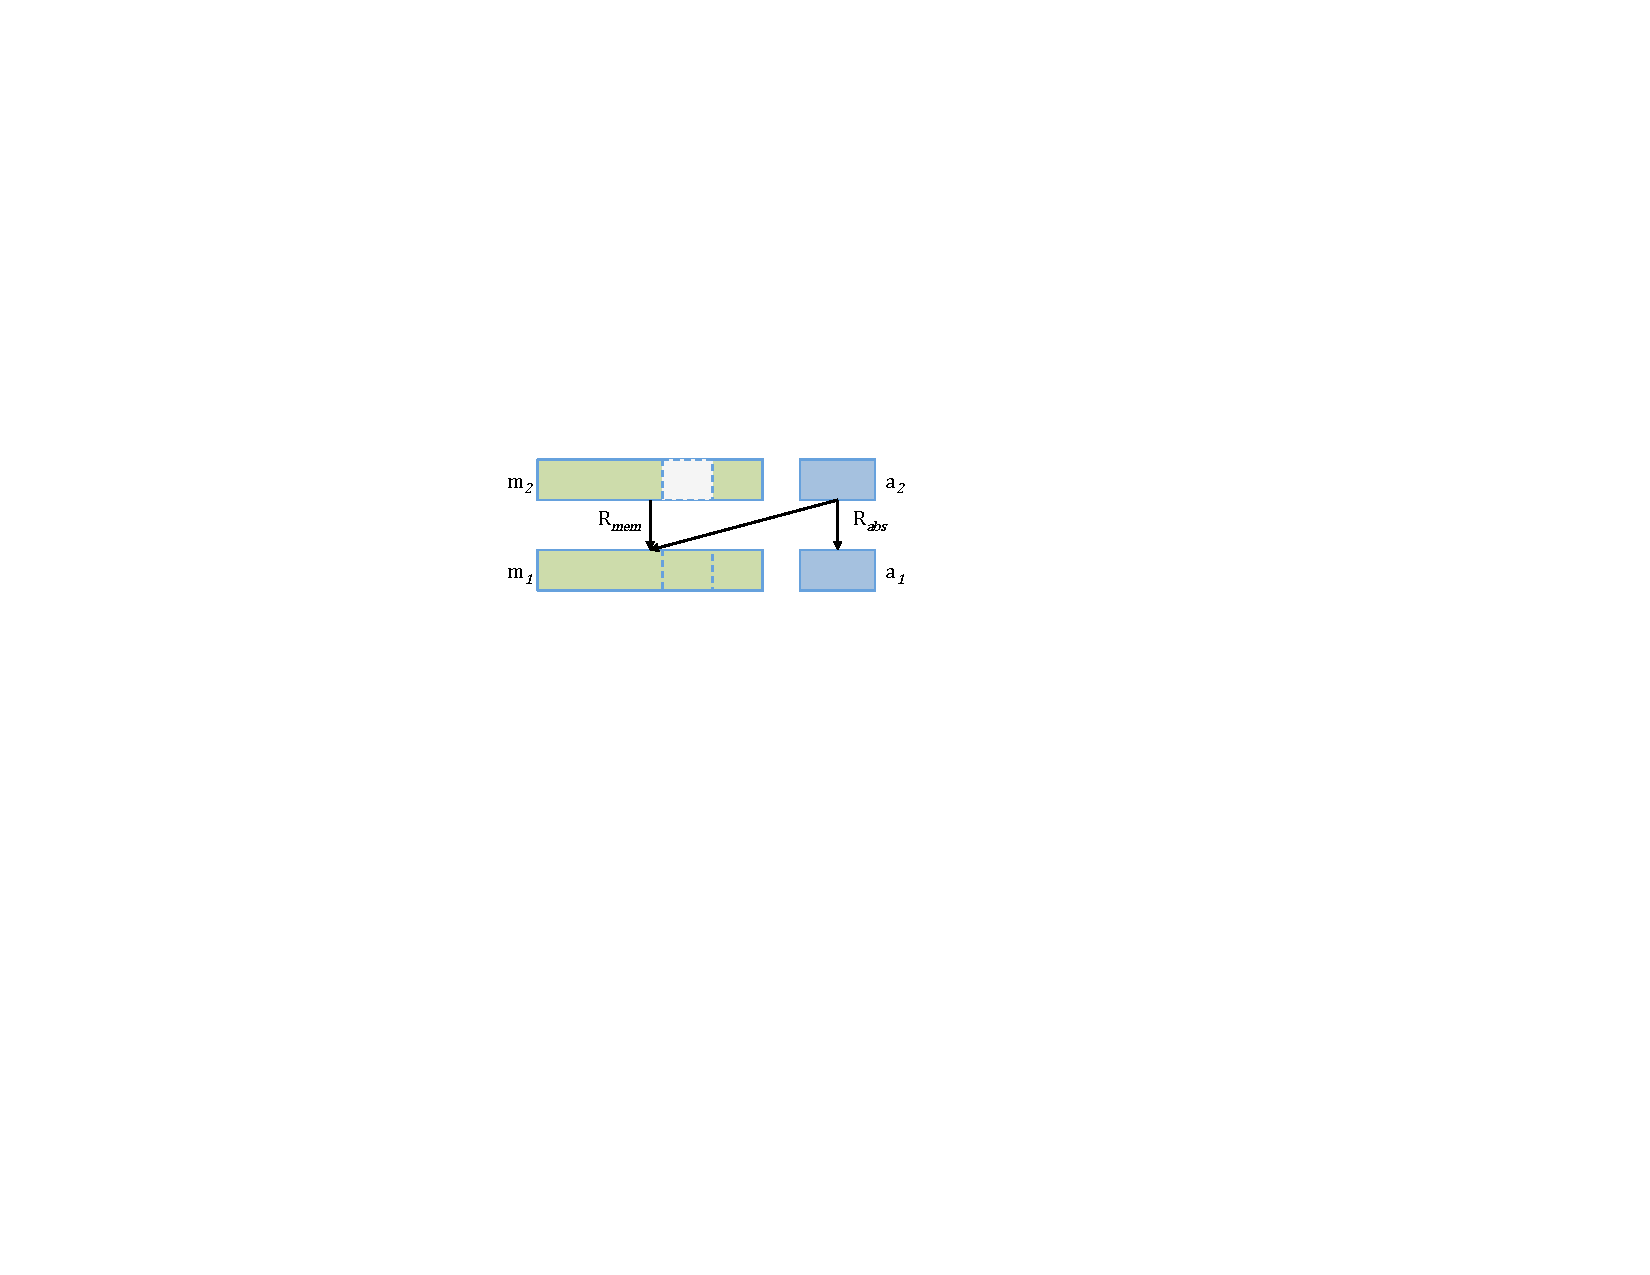
\includegraphics[scale=.7]{figs/layersimulation}
\caption{Layer simulation relation}
\label{fig:layersimulation}
%\vspace*{-7pt}
\end{center}
\afterpage{\FloatBarrier}
\end{figure}

To construct a certified abstraction layer $\layer{L_1}{M}{L_2}$, we
need to find a simulation $R$ such that $\ltyp{L_1}{R}{M}{L_2}$ holds.
Fig.~\ref{fig:lprooftree} gives an overview of this process.  We write
$M = \bigoplus_i i \mapsto \kappa_i$, where $i$ ranges over the
function identifiers defined in module $M$, and $\kappa_i$ is the
corresponding implementation.  Global variables in $M$ should not
be accessible from the layers above: their permissions are removed in
the overlay interface $L_2$.  The interface $L_2$ also includes a
specification $\sigma_i$ for each function $i$ defined in $M$.

We decouple the task of code verification from that of data structure
abstraction. We introduce an intermediate layer interface, $L_1'=\bigoplus_i i \mapsto \sigma'_i$, with its specifications
$\sigma'_i$ expressed in terms of the underlay states.
%%
We first prove that $\ltyp{L_1}{\id}{M}{L_1'}$ holds.  For each
function $i$ in $M$, we show that its implementation $\kappa_i$ is a
downward simulation of its ``underlay'' specification $\sigma'_i$,
that is, $\ltyp{L_1}{\id}{i \mapsto \kappa_i}{i \mapsto
  \sigma'_i}$. We apply the \rulename{Hcomp} rule to compose all the
per-function simulation statements.  Note the simulation
relations here are all \id, meaning there is no abstraction of
data structures in these steps.
%
% This downward simulation can be turned into an upward
% simulation because ClightX is determinate and receptive.  The
% downward simulation proof is sufficient here because the whole
% refinement proof between two layer interfaces is based on downward
% simulation, which will then be turned into an upward simulation at the
% level of whole-machine contextual refinement.
% 
We then prove $L_2 \lpath{R} L_1'$, which means that each specification
$\sigma_i$ in $L_2$ is an abstraction of the intermediate specification
$\sigma'_i$ via a simulation relation $R$.  
From $i \mapsto \sigma_i \lpath{R} i \mapsto \sigma'_i$,  
we apply the monotonicity rule \rulename{LLe-Mon} to 
get $L_2 \lpath{R} L_1'$. Finally, we apply the \rulename{Conseq} rule
to deduce $\ltyp{L_1}{R}{M}{L_2}$. 

%\vspace*{-3pt}
\paragraph{Verifying ClightX functions}
$L_1$ and $L_1'$ share the same views of both concrete and abstract states,
so no simulation relation is involved during this step of verification
(the \rulename{Fun} rule in Sec.~\ref{ssec:layer-langsem}).
Using Coq's tactical language,
we have developed a proof automation engine
that can handle most of the functional correctness proofs of
ClightX programs. It contains two main parts: a ClightX
statement/expression interpreter that generates the verification
conditions by utilizing rules of ClightX big-step semantics,
and an automated theorem prover that discharges
the generated verification conditions on the fly. 
The automated theorem prover is a first order prover,
extended with different theory solvers, such as the theory
of integer arithmetic and the theory of CompCert style partial maps.
The entire automation engine is developed in Coq's Ltac language.


In particular, the arithmetic theory solver is heavily invoked by the
prover. The semantics of Clight requires every value of intermediate
integer expressions to be in the appropriate range of its type. These
expressions may involve regular arithmetic operations such as
addition, subtraction, multiplication and division, but also more
complicated bit-wise operations such as shift, bit-wise and, or, and
complement. The built-in Coq tactic $omega$, which is used to
discharge arithmetic subgoals, is restricted to integer linear
arithmetic formulas, and thus are far from sufficient to deal with
complex formulas in our setting.


%\vspace*{-3pt}
\paragraph{Data abstraction}
Since primitives in $L_1'$ and $L_2$ are atomic, we prove the
single-step downward simulation between $L_1'$ and $L_2$ only at the
specification level.  The simulation proof for the abstraction can be
made language independent.  The simulation relation $R$ captures the
relation between the underlay state (concrete memory and abstract
state) and the overlay state, and can be decomposed as $R_\text{mem}$
and $R_\text{abs}$ (see Fig.~\ref{fig:layersimulation}). The relation
$R_\text{mem}$ ensures that the concrete memory states $m_1$ and $m_2$
contain the same values, while making sure the memory permissions for
the part to be abstracted are erased in the overlay memory $m_2$.  The
component $R_\text{abs}$ relates the overlay abstract state $a_2$ with
the full underlay state $(m_1, a_1)$.

Through this decomposition, we achieve the following two objectives:
the client program can directly manipulate the abstract state without
worrying about its underlying concrete implementation (which is hidden
via $R_\text{mem}$), and the abstract state in the overlay is actually
implementable by the concrete memory and abstract state in the
underlay (via $R_\text{abs}$).

%%%%%%%%%%%%%%%%%%%%%%%%%%%%%%%%%%%%%%%%%%%%
\begin{figure}[t]\scriptsize
$$
\begin{array}{l|l}
\hspace*{-2ex}
\begin{array}[t]{l}
\verb+typedef enum {+\\
\verb+  PG_RESERVED, PG_KERNEL,+\\
\verb+  PG_NORMAL+\\
\verb+} pg_type;+\\
\\
\verb+struct page_info {+\\
\verb+  pg_type	t;+\\
\verb+  uint	u;+\\
\verb+};+\\
\verb+struct page_info AT[1<<20];+
\end{array}
&
\begin{array}[t]{l}
\verb+Notation RESV := 0.+\\
\verb"Notation KERN := (RESV + 1)."\\
\verb"Notation NORM := (KERN + 1)."\\
\\
\verb+Inductive page_info :=+\\
\verb+| ATV (t: Z) (u: Z)+\\ 
\verb+| ATUndef.+\\
\\
\verb+Record abs'' :=+\\
\verb+  {AT: ZMap.t page_info}.+\\
\end{array}
\end{array}
$$ 
\caption{Concrete (C) vs. abstract (Coq) memory allocation table}
\label{fig:alt}
\end{figure}

\begin{figure}[t]\scriptsize
$$
\begin{array}{l|l}
\hspace*{-3ex}
\begin{array}[t]{l}
\verb+// +\kappa_\textsf{at\_get}\\
\verb+uint at_get (uint i){+\\
\verb+  uint allocated;+\\
\verb+  allocated = AT[i].u;+\\
\verb+  if (allocated != 0)+\\
\verb+      allocated = 1;+\\
\verb+  return allocated;+\\
\verb+}+\\
\\
\verb+// +\kappa_\textsf{at\_set}\\
\verb+void at_set (uint i, uint b){+\\
\verb+    AT[i].u = b;+\\
\verb+}+
\end{array}
&
\begin{array}[t]{l}
\verb+Function + \hat{\sigma}_\textsf{at\_get} \verb+ a i :=+\\
\verb+match (a.AT i) with+\\
\verb+| ATV _ 0 => Some 0+\\
\verb+| ATV _ _ => Some 1+\\
\verb+| _ => None+\\
\verb+end.+\\
\\
\verb+Function + \hat{\sigma}_\textsf{at\_set} \verb+ a i b :=+\\
\verb+match (a.AT i) with+\\
\verb+| ATV t _ =>+\\
\verb+Some (set_AT a i (ATV t b))+\\
\verb+| _ => None+\\
\verb+end.+
\end{array}
\end{array}
$$ 
\caption{Concrete vs. abstract getter-setter functions for \textsf{AT}}
\label{fig:alt:gettersetter}
\end{figure}
 
\begin{figure}[t]\scriptsize
$$
\begin{array}{l|l}
\begin{array}[t]{l}
\verb+Inductive +\sigma'_\textsf{at\_set}\verb+ :=+\\
\verb"| "\forall\verb+ m m' a ofs v n,+\\
\verb+   m.store AT ofs v = m'+\\
\verb"  ->"\verb" ofs = n * 8 + 4"\\
\verb"  ->"\verb" 0 <= n < 1048576"\\
\verb"  ->"\verb" "\sigma'_\textsf{at\_set}\verb" (n::v::nil)"\\
\verb"        m a Vundef m' a."
\end{array}
&
\begin{array}[t]{l}
\verb+Inductive +\sigma_\textsf{at\_set}\verb+ :=+\\
\verb"| "\forall\verb+ m a a' n v,+\\
\verb+   +\hat{\sigma}_\textsf{at\_set}\verb+ a n v = Some a'+\\
\verb"  ->"\verb" 0 <= n < 1048576"\\
\verb"  -> "\sigma_\textsf{at\_set} \verb" (n::v::nil)"\\
\verb"       m a Vundef m a'."
\end{array}
\end{array}
$$ 
\caption{High level and low level specification for \textsf{at\_set}}
\label{fig:alt:spec}
\end{figure}

%\vspace*{-3pt}
\paragraph{Common patterns}
We have developed two common design patterns to further ease the task of
verification. The {\it getter-setter} pattern establishes memory
abstraction by introducing new abstract states and erasing
the corresponding memory permissions for the overlay.
The overlay only adds the \textsf{get}
and \textsf{set} primitives which are implemented using simple
memory load/store operations at the underlay.
The {\it abs-fun} pattern implements key functionalities, but does not
introduce new abstract state. Its implementation (on underlay) does
not touch concrete memory state. Instead, it only accesses the states
that have already been abstracted, and it only does
so using the primitives provided by the underlay interface.

Figs.~\ref{fig:alt}-\ref{fig:palloc:spec} show how we use the two
patterns to implement and verify a simplified physical memory
allocator $\textsf{palloc}$, which allocates and returns the
first free entry in the physical memory allocation table.
Fig.~\ref{fig:alt}-\ref{fig:alt:spec} shows how we follow
the {\it getter-setter} pattern
to abstract the allocation table into a new abstract state.
As shown in Fig.~\ref{fig:alt}, we first turn the concrete C
memory allocation table implementation into an abstract Coq data
type. Then we implement the getter and setter functions for the
memory allocation table, both in C and Coq (see Fig.~\ref{fig:alt:gettersetter}). 
The Coq functions $\hat{\sigma}_\textsf{at\_get}$ and $\hat{\sigma}_\textsf{at\_set}$
are just intermediate specifications that are used
later in the overlay specifications.
The actual underlay and overlay specifications of the setter
function $\textsf{at\_set}$ are shown in Fig.~\ref{fig:alt:spec}.

We then prove
$\ltyp{L_1}{\id}{\textsf{at\_set} \mapsto \kappa_\textsf{at\_set}}{\textsf{at\_set} \mapsto \sigma'_\textsf{at\_set}}$,
and also 
$\textsf{at\_set} \mapsto \sigma_\textsf{at\_set}\lpath{R}\textsf{at\_set} \mapsto \sigma'_\textsf{at\_set}$.

\begin{figure}[t]\scriptsize
$$
\begin{array}{l|l}
\hspace*{-3ex}
\begin{array}[t]{l}
\verb+// +\kappa_\textsf{palloc}\\
\verb+uint palloc(uint nps){+\\
\verb+  uint i = 0, u;+\\
\verb+  uint freei = nps;+\\
\verb+  while(freei == nps+\\
\verb+         && i < nps) {+\\
\verb+     u = at_get(i);+\\
\verb+     if (u == 0)+\\
\verb+       freei = i;+\\
\verb"     i ++;"\\
\verb+  }+\\
\verb+  if (freei != nps)+\\
\verb+    at_set(freei, 1);+\\
\verb+  return freei;+\\
\verb+}+\\
\end{array}
&
\begin{array}[t]{l}
\verb+Definition first_free a n:+\\
\verb+  {v| 0<= fst v < n+\\
\verb+   /\+\verb+ a.AT (fst v) = ATV (snd v) 0+\\
\verb+   /\+\verb+ +\forall\ \verb+x, 0 <= x < fst v+\\
\verb+       -> +\sim\verb+a.AT x = ATV _ 0}+\\
\verb"+ {"\forall\ \verb+x, 0 <= x < n+\\
\verb+       -> +\sim\verb+a.AT x = ATV _ 0}.+\\
\\
\verb+Function + \hat{\sigma}_\textsf{palloc} \verb+ a nps :=+\\
\verb+match first_free a nps with+\\
\verb+ | inleft (exist (i, t) _) =>+\\
\verb+   (set_AT a i (ATV t 1), i)+\\
\verb+ | _ => (a, nps)+\\
\verb+end.+\\
\end{array}
\end{array}
$$ 
\caption{Concrete (in C) vs. abstract (in Coq) \textsf{palloc} function}
\label{fig:palloc}
\end{figure}

\begin{figure}[t]\scriptsize
$$
\begin{array}[t]{l}
\verb+Inductive +\sigma'_\textsf{palloc}\verb+ : spec :=+\\
\verb"| "\forall\verb+ m a a' nps n,+\\
\verb+   +\hat{\sigma}_\textsf{palloc}\verb+ a nps = (a', n)+\\
\verb"  -> 0 <= nps < 1048576"\\
\verb"  -> " \sigma'_\textsf{palloc}\verb" (nps::nil) m a n m a'."\\
\\
\verb"Definition "\sigma_\textsf{palloc}\verb" := "\sigma'_\textsf{palloc}.   
\end{array}
$$ 
\caption{High level and low level specification for palloc function}
\label{fig:palloc:spec}
\end{figure}

%%%%%%%%%%%%%%%%%%%%%%%%%%%%%%%%%%%%%%%%%%%%

The code verification (first part) is easy for this pattern
because the memory load and store operations in the underlay
match the source code closely.
The proof can be discharged by our automation tactic.
The main task of this pattern is to prove refinement (second part):
we design a simulation relation $R$
relating the memory storing the global variable at underlay
with its corresponding abstract data at overlay.
The component $R_\text{mem}$ ensures that there is no permission
for allocation table \verb"AT" in overlay memory state $m_2$, 
while the component $R_\text{abs}$ is defined as follows:
\begin{itemize}%[noitemsep,nolistsep]
\item $\forall i \in [0, 2^{20})$, $R_\text{abs}$ enforces the {\em writable}
permission on \verb"AT[i]" at underlay memory state $m_1$, and requires
($a_2$.\verb"AT"  \verb"i") at overlay to be
\verb"(ATV AT[i].t AT[i].u)".

\item Except for \verb"AT", $R_\text{abs}$ requires all other abstract data in
underlay and overlay to be the same.
\end{itemize}
The refinement proof for $L_2 \lpath{R} L_1'$ involves the efforts to
prove that this relation $R$ between underlay memory and overlay
abstract state is preserved by all the atomic primitives in both $L_1'$ and $L_2$.

After we abstract the memory and get/set operations,
%of the allocation table
we implement $\textsf{palloc}$ on top of $L_2$,
following the {\it abs-fun} pattern.
The previous overlay now becomes the new underlay (``$L_1$'').
Fig.~\ref{fig:palloc} shows both the implementation of
$\textsf{palloc}$ in ClightX and the abstract function in Coq.
As before, we separately show that
$\ltyp{L_1}{\id}%
	{\textsf{palloc} \mapsto \kappa_\textsf{palloc}}%
	{\textsf{palloc} \mapsto \sigma'_\textsf{palloc}}$,
and 
$\textsf{palloc} \mapsto \sigma_\textsf{palloc}\lpath{R}
\textsf{palloc} \mapsto \sigma'_\textsf{palloc}$
holds.
For the {\it abs-fun} pattern, the refinement proof is easy.
Since we do not introduce any new abstract states in this pattern,
the implementation only manipulates the abstract states through the
primitive calls of the underlay. Thus, as shown in Fig. \ref{fig:palloc:spec},
the corresponding underlay and overlay specifications are exactly the same,
so the relation $R$ here is the identity (\id) and 
the proof of refinement is trivial.
The main task for the {\it abs-fun}
pattern is to verify the code, which is done using our automation tactic. 


Due to the presence of a loop in the C code (see Fig.~\ref{fig:palloc}), 
the automation tactic is not able to automate the proofs completely.
Since the big-step semantics only specifies the infinite loop,
naive applications of the semantic constructors of loops as
logical rules lead to an infinite sequence of applications.
In our framework, we introduce a separate inference rule as a
lemma for proving both the correctness and the termination of the loops.
The lemma requires the prover to provide both the loop invariants
(for partial correctness) and the loop variant (for termination).
Once the right loop invariants and variant are provided, the proof
can be mostly automated using our proof automation engine.


The above examples show that for the {\it getter-setter} pattern, the
primary task is to prove data abstraction, while for the {\it abs-fun}
pattern, the main task is to do simple program verification.  These
two tasks are well understood and manageable, so the decoupling (via
these two patterns) makes the layer construction much easier. 


It means that although
the proof of $\ltyp{L_1}{R}{M}{L_2}$ is separated into two disjoint
tasks, by following the two patterns, the proof is merely focused
on one of them.



\paragraph{Verification of Functional Correctness}

Verification of ClightX code is done on a per-function basis.
For each function $f$ implemented on top of layer interface $L$, we write a deep specification
$f_S$ of the form $f_S(args,m,a,res, m',a')$, which precisely capture
the change of states by $f$ from $(m, a)$ into $(m', a')$ with
return value $res$ when executed with arguments $args$.
Then we prove a downward simulation relation between $f_S$ and $f$,
which can be turned into the upward simulation, i.e., the proof
that the implementation is the refinement of the specification,
due to the fact that the semantics of the $ClightX(L)$ is deterministic.
However, the downward simulation proof is enough in our case,
in the sense that we do not need to turn downward simulation into upward simulation,
because the whole refinement proof between two layer interfaces is based on downward simulation,
which is in turn turned into an upward simulation at the level of whole-machine contextual
refinement.

For example, show dequeue refinement theorem here...

To prove the above theorem, we have developed a powerful proof automation
engine for the language ClightX, all in Coq's tactical language.
It directly utilizes the constructors of the CompCert ClightX big-step
semantic rules to interpret the statements of the function body, while
using it's back-end theorem proving engines to automatically discharge
the verification conditions generated by applying the semantic constructors.

Talk about the verification condition generation here...

Talk about the tautology solver, advanced arithmetic theory solver, term rewritter and so on...

This is possible thanks to the analogy between the deep specification and the concrete
implementation.



\paragraph{Establishing Invariants}
Global variables usually require stating and proving some invariant properties.
For example, in operating system design, thread queues are normally implemented
as doubly-linked lists. The corresponding invariants might state that,
\begin{invariant}
\begin{enumerate}
\item The queue is well formed, i.e., all forward and back links in the list
point to the appropriate node (except the head and tail).
\item Non-active threads are not in any of the thread queue.
\item All active threads appear in one and exactly one thread queue.
\item Each thread can appear in a queue at most once.
\item Each queue only contains active threads.
\end{enumerate}
\end{invariant}
Invariants are expensive because they need to be proved not only
locally for the functions manipulating the variables, but also for the whole system,
e.g., need to show that no other pointer manipulations in the system
destroy the invariant properties. 
In other words, invariants are the global properties that are expected to hold
in any execution of the program.
Furthermore, sometimes, some functions have
to temporarily break the invariants. For example, the \verb+dequeue+ operator,
which removes a node from the doubly linked list, temporarily breaks the invariants
by allowing the queue to be temporarily ill formed in the middle of execution.
In complex systems like operating system kernel, proofs on invariants are even
trickier, as you not only need to show the invariants hold on the kernel implementation,
but also during the execution of any client/user programs.
For the seL4 project, though they prove the properties of kernel source code alone,
they mention that 80\% of their initial efforts in the
refinement proofs went into establishing invariants, and only 20\% into the
actual functional correctness proof \cite{klein2009sel4}.

In the verification of the \mCTOS{} (see Section \ref{sec:kernel}),
we take a novel approach, which we believe significantly eased the task of invariant
related proofs. 
First, we never enforce any explicit invariants on the raw memory. All the kernel data
structures in the memory are first abstracted into logical states. And all the
invariants are stated in terms of those abstract data. Recall the only way
a ClightX program interacts with abstract data is by calling the primitives.
At each layer interface $L$, we state the invariants $inv(L)$ strictly on the abstract
data of $L$, and show a global property that the invariants hold at any execution
point of any programs running on $L$. This is achieved by showing the initial
abstract data satisfies the invariants, and all the primitives of $L$ preserve
the invariants of $L$. 
Thanks to this global property, during a verification of the functional correctness
of function $f$ implemented on top of layer interface $L$, you get free access to use all the invariants
of $L$ as facts. It also exempt you completely from worrying about invariants
related proofs during the proof of functional correctness of $f$.
During the verification of $f$, there is no need
to prove anything related to invariant preservation, cause it is already proved globally
that whatever the function does, the invariants are preserved.

The function $f$ verified on top of the underlay $L$ may get exposed as an abstract primitive to
the overlay. The overlay may have a completely different set of layer invariants,
and you just need to prove that the abstract specification of the function preservers
the invariants of the overlay, to achieve the global invariants property of the
overlay.
For example, you may implement a setter/getter on top of underlay $L$, which reads and writes to
a piece of memory. We do not enforce any invariants on that piece of memory. At the
overlay, that memory is abstracted into an abstract data type, and we show that
the abstract specifications of setters and getters (which reads and writes to the
abstract states instead), preserve the invariants of that overlay.

This new approach has following advantages:
\begin{itemize}
\item For each layer interface $L$, invariant proofs are done globally once and for all.
This let us focus on the main functional correctness proofs.
\item Invariant preservation proofs are always on abstract specifications, which
are atomic. You no longer need to worry about the actual implementation of the
function temporarily breaks the invariants in the middle of the execution.
\item Postpone the introduction of invariants to the right layer interface.
We introduce the last 4 invariants of the thread queue implementation above
only when we get to the most abstract view shown in the Example ?.
This means, those invariants are no longer proved on complicated initial or
intermediate representations of the thread queues, but only proved with
the most abstract specifications, where a thread queue is interpreted as a
Coq list.
\item Better isolation. The invariants on abstract data that is not modified
by an abstract specification is trivially satisfied.
\item Hiding primitives. The second invariants above can easily be violated
if you simply call a primitive to inactivate or free a thread in a queue
before popping the queue out of the thread. But when we introduce the
invariants we hide the corresponding low level primitives that directly
activates/deactivates threads, enqueue, dequeue, and expose a more higher
level primitive \verb+thread_free+, which both deactivates a thread and
pops the thread out of the queue. Since the primitive execution is atomic,
this does not break any invariants of the layer interface. In a word, when we introduce
new invariants that potentially get broken by previous low level primitives,
we implement and expose only new high level primitives that respects the
invariants. This restricts the context program to only those that respects
our invariants.
\item Hiding the invariants. Once the virtual memory manager is implemented,
there is no need to expose the low level physical memory allocation table
any more to the overlay or the higher layers. When we hide the corresponding abstract
data and primitives, we also remove corresponding invariants on the data
as well. Fewer number of invariants means fewer proof efforts needed.
\end{itemize}




\begin{figure}[t]\scriptsize
$$
\begin{array}{l}
\begin{array}{l}
\verb+struct pmap {+\\
\verb+  alignas(4096) uint pdir[1024];+\\
\verb+  alignas(4096) uint pt[1024][1024];+\\
\verb+};+\\
\verb+alignas(4096) struct pmap pmp[64];+\\
\\
\verb+void set_PTX(uint pid, uint pde, uint pte,+\\
\verb+             uint paddr, uint perm){+\\
\verb"  pmp[pid].pt[pdx][ptx] = paddr + perm;"\\
\verb+}+
\end{array}
\\
\hline
\\
\begin{array}{l}
\verb+Inductive PTPerm: Type := |PTE_P |PTE_W |PTE_U.+\\
\verb+Inductive PTInfo:=+\\
\verb+  |PTValid (v: block)(p: PTPerm) |PTUnPresent |PTUndef.+\\
\verb+Definition pt := ZMap.t PTInfo.+\\
\verb+Inductive pdir := |PDTValid (pte: pt) |PDTUndef.+\\
\verb+Definition pmap := ZMap.t pdir.+\\
\verb+Definition pmp := ZMap.t pmap.+
\end{array}
\end{array}
$$ 
\caption{Concrete (in C) vs. abstract (in Coq) page maps}
\label{fig:pmap}
%\vspace*{-7pt}
\end{figure}



\section{Layered Programming in LAsm}
\label{sec:seq:lasm}

In this section, we describe LAsm, the \emph{Layered
  Assembly language}, and the extended machine model which LAsm is based on.

The reason we are interested in assembly code and behavior is
threefold.  First of all, even though we provide ClightX to write most
code, we are still interested in the actual assembly code running on
the actual machine. In Section \ref{sec:seq:comp}, we will provide a
verified compiler to transport all proofs of code written in ClightX
to assembly.

\begin{figure}[t]\centering
\lstinputlisting [language = C, multicols=2] {source_code/seq-cswitch.c}
\caption{Kernel context switch verified in LAsm}
\label{fig:contextswitch}
\hrulefill
\end{figure}

Secondly, there are parts of software that have to be manually written
in assembly for various reasons. For example, the standard
implementation of kernel context switch, shown in
Figure~\ref{fig:contextswitch}, 
modifies the stack pointer register
\textsf{ESP}, which does not satisfy the C calling convention and has
to be verified in assembly.  A linker will be defined in Section
\ref{sec:seq:comp} to link them with compiled C code.

Last but not least, we are interested not only in the behavior of our
code, but also in the behavior of the \emph{context} that will call
functions defined in our code. To be as general as possible, we allow
the context to include all valid assembly code sequences. To this end,
it is necessary to transport per-function refinement proofs to a
whole-machine \emph{contextual refinement} proof.


  \subsection{LAsm and layer interfaces}

We start from the syntax and formal semantics of the 32-bit x86
assembly subset specified in CompCert.
CompCert x86 assembly is
modeled as a state machine with a register set and a memory state. 
The register set
consists of eight 32-bit general-purpose registers and eight XMM registers
designated as scalar double-precision floating-point operands.
The memory state is same as the one in Clight.
In particular, each function executes with its stack frame modeled in its
own memory block, so that the stack is not a contiguous piece of
memory.
Another anomaly regarding function calls in CompCert x86 assembly is that
the return address is stored in pseudo-register $\mathsf{RA}$ instead of
being pushed onto the stack, so
that the callee must allocate its own stack frame and
store the return address 
using the \textsf{Pallocframe} and
\textsf{Pfreeframe} pseudo-instructions.

\begin{figure}[t]\centering
\[
\begin{array}{llll}
\mathit{ri}  & ::= & \mathsf{ESP} \, | \mathsf{EBP} \, & \text{Stack registers} \\
& | & \mathsf{EAX} \, | \mathsf{EBX} \, | \mathsf{ECX} \, | \mathsf{EDX} & \text{Integer registers} \\
\mathit{rf} & ::= & \mathsf{FP0} \, | \mathsf{XMM0} \, | \mathsf{XMM1} \dots | \mathsf{XMM7} & \text{Floating-point registers} \\
r & \in & \textsf{preg} & \text{Registers} \\
 & ::= & \mathit{ri} \, | \mathit{rf} \\
& | & \mathsf{EIP} \, | \mathsf{RA} & \text{Prog counter, return addr} \\
\end{array}
\]
\[
\begin{array}{llll}
\mathit{ti} & ::= & \mathit{ri} & \text{Direct integer register access} \\
& | & (\mathit{ri})n & \text{Indirect load/store via int register} \\
& | & x+n & \text{Load/store to global variable} \\
\mathit{si} & ::= & \mathit{ti} & \text{Dereference} \\
& | & \$n & \text{Constant integer} \\
& | & \$x+n & \text{Pointer to global variable} \\
\\
\mathit{tf} & ::= & \mathit{rf} \, | (\mathit{ri})n \, | x+n & \text{Floating-point targets} \\
\mathit{sf} & ::= & \mathit{tf} \, | \$q \, & \text{Floating-point sources} \\
\\
\mathit{I} & ::= & \mathtt{movi} ~ \mathit{si}, \mathit{ti} & \text{Integer move/load/store} \\
& | & \mathtt{leai} ~ \mathit{si}, \mathit{ti} & \text{Integer load/store from address} \\
& | & \mathtt{movf} ~ \mathit{sf}, \mathit{tf} & \text{Floating-point move/load/store} \\
& | & \mathtt{addi} ~ \mathit{ri}_d, \mathit{ri}_o & \text{Arithmetic} \\
& | & \mathtt{subi} ~ \mathit{ri}_d, \mathit{ri}_o \, | \dots \\
& | & \mathtt{call} ~ \mathit{ti} \, | \mathtt{ret} & \text{Function call and return} \\
& | & \mathtt{push} ~ \mathit{ri} \, | \mathtt{pop} ~ \mathit{ri} & \text{Regular register push/pop} \\
& | & \mathsf{Pallocframe} ~ n & \text{Allocate stack frame} \\
& | & \mathsf{Pfreeframe} ~ n & \text{Free stack frame}
\end{array}
\]
\caption{The syntax of LAsm}
\label{fig:seq:lasm:syntax}
\hrulefill
\end{figure}

Similarly to ClightX, we extend the machine state with an abstract
state, which will be modified by primitives. This yields LAsm, whose
syntax (\cf Figure~\ref{fig:seq:lasm:syntax}) is the same as that of CompCert x86 assembly, except that the
semantics will be parameterized over the type of abstract states and
the specifications of primitives.  Most notably, primitive calls are
syntactically indistinguishable from normal function calls, yet depend
on the specifications semantically.

Moreover, in our Coq formalization, the semantics of LAsm is also
equipped with \emph{memory accessors} for address translation in order to handle both
kernel memory linear mapping and user space virtual memory.
In the latter case, plain integers can be treated
as pointers to user memory, as opposed to kernel memory modeled as the
CompCert-style concrete memory state. 

\begin{definition}[LAsm Modules]
A LAsm module is a finite map from identifiers to arrays of LAsm
instructions.
\end{definition}

\ignore{We define the semantics of LAsm in small-step form. The machine
state is $(\rho, m, a)$ where $\rho$ contains the values of registers,
$m$ is the concrete memory state and $a$ is the abstract state. Let
$M$ be an LAsm module, which is a finite map from identifiers to arrays of LAsm
instructions, we write $\Gamma, L, M \vdash (\rho, m, a)
\rightarrow (\rho', m', a')$ a transition step in the LAsm machine. The full syntax and formal semantics of LAsm is described in the
  companion technical report.}

\ignore{
\begin{figure}[t]\scriptsize
$$
\begin{array}{l|l}
\begin{array}{l}
\verb+kctxt_switch:+\\
\verb+	leai	0(%eax,%eax,2), %eax+\\
\verb+	leai	KCtxtP(,%eax,8), %eax+\\
\verb+	movi	%esp, 0(%eax)+\\
\verb+	movi	%edi, 4(%eax)+\\
\verb+	movi	%esi, 8(%eax)+\\
\verb+	movi	%ebx, 12(%eax)+\\
\verb+	movi	%ebp, 16(%eax)+\\
\verb+	pop	%ecx+\\
\verb+	movi	%ecx, 20(%eax)+\\
\verb+	leai	0(%edx,%edx,2), %edx+
\end{array}
&
\begin{array}{l}
\\
\verb+	leai	KCtxtP(,%edx,8), %edx+\\
\verb+	movi	0(%edx), %esp+\\
\verb+	movi	4(%edx), %edi+\\
\verb+	movi	8(%edx), %esi+\\
\verb+	movi	12(%edx), %ebx+\\
\verb+	movi	16(%edx), %ebp+\\
\verb+	movi	20(%edx), %ecx+\\
\verb+	push	%ecx+\\
\verb+	xor	%eax, %eax+\\
\verb+	ret+\\
\verb+......+
\end{array}
\end{array}
$$
\caption{Kernel context switch verified in LAsm}
\label{fig:contextswitch}
\end{figure}
}

%\vspace*{-3pt}
\paragraph{Assembly layer interfaces}
The semantics of LAsm is parameterized over a layer interface.
Different from C-style primitives (\cf Definition~\ref{def:c-prim}), which are defined using
argument list and return value, primitives implemented in LAsm
often utilize their full control over the
register set and are not restricted to a particular calling convention (\eg, context switch).
Therefore, it is necessary to extend the structure of layer
interfaces to allow assembly-style primitives modifying the register set.

\begin{definition}[Assembly-style primitive]
An assembly-style primitive specification $P$ over the abstract state type
$\abst$ is a predicate on $((\textsf{preg} \rightarrow \textsf{val}) \times \textsf{mem} \times \abst) \times
((\textsf{preg} \rightarrow \textsf{val}) \times \textsf{mem} \times \abst)$. $P(\rho, m, a,
\rho', m', a')$ says that the primitive $P$ takes
register set $\rho$, memory state $m$ and abstract state $a$ as
arguments, and returns register set $\rho'$, memory state
$m'$ and abstract state $a'$ as result.
\end{definition}

By ``\emph{style},'' we mean the calling convention,
not the language in which they are actually implemented.
C-style primitives may very well be implemented as hand-written
assembly code at underlay.

We can then define assembly layer interfaces by replacing the primitive
specification with our assembly-style one in Definition~\ref{def:c-layer}.
But, to make reasoning simpler, when defining assembly layer interfaces,
we distinguish C-style from assembly-style primitives.
First, C-style primitives
can be refined by other C-style primitives. 
Second and most importantly, it
becomes possible to instantiate the semantics of ClightX with an
\emph{assembly} layer interface by just considering C-style primitives and ignoring
assembly-style primitives (which might not follow the C calling convention).
In this way, ClightX code is only allowed to call C-style
primitives, whereas LAsm can actually call both kinds of primitives.

\begin{definition}[Assembly layer interface] \label{def:asm-layer}
An assembly layer interface $L$ is a tuple
$ L = (\abst, \primt_{\mathrm{ClightX}}, \primt_{\mathrm{LAsm}}, \invt, \mat) $
where:
\begin{itemize}
\item $(\abst, \primt_{\mathrm{ClightX}}, \invt)$ is a C layer interface (\cf
Definition~\ref{def:c-layer})
\item $\primt_{\mathrm{LAsm}}$ is a finite map from identifiers to assembly-style
primitive specifications over the abstract state $\abst$. The domains of
$\primt_{\mathrm{ClightX}}$ and $\primt_{\mathrm{LAsm}}$ shall be disjoint.
\item $\mat$ is the memory accessor used for address translation.
\end{itemize}
\end{definition}


\paragraph{Small-step semantics}

We write $\llbracket \mathit{ti} \rrbracket^\triangleleft(\Gamma, \rho)$
(\emph{resp}. $\llbracket \mathit{tf} \rrbracket^\triangleleft(\Gamma, \rho)$)
to denote the evaluation of integer (\emph{resp}. floating-point) registers
and global variables as targets for \texttt{mov} operations, where
$\Gamma$ is a mapping from global variables to memory block
identifiers, and $\rho$ is a mapping from registers to values.

\[
\begin{array}{lll}
\llbracket (\mathit{ri})n \rrbracket^\triangleleft(\Gamma, \rho) & = (n' + n) & \text{if} ~ \rho(\mathit{ri}) = n' \\
\llbracket (\mathit{ri})n \rrbracket^\triangleleft(\Gamma, \rho) & = (b, \mathit{ofs}+n) & \text{if} ~ \rho(\mathit{ri}) = (b, \mathit{ofs}) \\
\llbracket x + n  \rrbracket^\triangleleft(\Gamma, \rho) & = (b, n) & \text{if} ~ \Gamma(x) = b
\end{array}
\]

To evaluate indirect load through registers and global variables as
source operand for $\mathtt{mov}$ operations, we write $\llbracket s
\rrbracket^\triangleright(\Gamma, \rho, m)$ the evaluation of
\texttt{mov} operands.

\[
\begin{array}{ll}
\llbracket s \rrbracket^\triangleright(\Gamma, \rho, m)  = m(v) &
\text{if }  \llbracket s \rrbracket^\triangleleft(\Gamma, \rho) = v 
\\
\llbracket r \rrbracket^\triangleright(\Gamma, \rho, m)= \rho(r) &
\llbracket \$ n \rrbracket^\triangleright(\Gamma, \rho, m)  = n 
\\
\llbracket \$ q \rrbracket^\triangleright(\Gamma, \rho, m)  = q 
\\
\llbracket \$ x+n \rrbracket^\triangleright(\Gamma, \rho, m)  = (b, n)  &
\text{if }  \Gamma(x)  = b 
\end{array}
\]

For any register set $\rho$, we write 
\[\mathsf{nextEIP}(\rho) =
\rho[\mathsf{EIP} \leftarrow (b, \mathit{ofs}+1)] \text{ if }\rho(\mathsf{EIP})
  = (b, \mathit{ofs})\]%
The register $\mathsf{EIP}$ is assumed to contain a
  pointer $(b, \mathit{ofs})$ where $b$ is the memory block
  corresponding to the current function, and $\mathit{ofs}$ is the
  index of the current instruction within this function; in the exact
  same way as in CompCert x86 assembly, we assume that all
  instructions are of size 1.

Function call and return only modify the value of registers \textsf{EIP} and \textsf{RA}.

Similarly to CompCert x86 assembly, \textsf{Pallocframe} allocates a
new stack frame memory block, stores the return address and a back
link to the parent stack frame, and makes the stack pointer point to
the new stack frame. Conversely, \textsf{Pfreeframe} restores the
previous values of the stack pointer and return address, then frees
the current stack block.

We define the semantics of LAsm in small-step form. The machine
state is $(\rho, m, a)$ where $\rho$ contains the values of registers,
$m$ is the concrete memory state and $a$ is the abstract state.  Let
$M$ be a module, we write $\Gamma, L, M \vdash (\rho, m, a)
\rightarrow (\rho', m', a')$ a transition step in the LAsm machine.

\begin{figure}[t]
\begin{mathpar}
\inferrule{
\llbracket s \rrbracket ^ \triangleright(\Gamma, \rho, m)  = v 
\\
\rho'  = \mathsf{nextEIP}(\rho[r \leftarrow v])
}
{\llbracket \mathtt{mov}~ s, r \rrbracket(\Gamma, L; \rho, m, a)  = (\rho', m, a)}
\and
\inferrule{
\llbracket s \rrbracket ^ \triangleright(\Gamma, \rho, m) = v_s
\\
\llbracket t \rrbracket ^ \triangleleft(\Gamma, \rho) = v_t\\
m' = m[v_t \leftarrow v_s]\\
\rho_2  = \mathsf{nextEIP}(\rho_1)
}
{\llbracket \mathtt{mov}~ s, t \rrbracket(\Gamma, L; \rho, m, a) = (\rho_2, m', a') }
\and
\inferrule{
\rho(r_s)  = n 
\\
\rho(r_t) = (b, \mathit{ofs}) 
\\
\rho' = \mathsf{nextEIP}(\rho[r_t \leftarrow (b, \mathit{ofs}+n)])
}
{\llbracket \mathtt{addi}~ r_s, r_t \rrbracket(\Gamma, L; \rho, m, a) = (\rho', m, a) }
\and
\inferrule{
\rho(r_s) = (b, \mathit{ofs}_s) 
\\
\rho(r_t) = (b, \mathit{ofs}_t) 
\\
\rho' = \mathsf{nextEIP}(\rho[r_t \leftarrow (\mathit{ofs}_t - \mathit{ofs}_s)])
}
{\llbracket \mathtt{subi}~ r_s, r_t \rrbracket(\Gamma, L; \rho, m, a) = (\rho', m, a) }
\and
\inferrule{
\llbracket t \rrbracket^\triangleleft(\Gamma, \rho)  = v
\\
\rho' = \rho[\mathsf{EIP} \leftarrow v][\mathsf{RA} \leftarrow \rho(\mathsf{EIP})] 
}
{\llbracket \mathtt{call} ~ t \rrbracket(\Gamma, L; \rho, m, a) = (\rho', m, a)}
\and
\inferrule{
\rho' = \rho[\mathsf{EIP} \leftarrow \rho(\mathsf{RA})][\mathsf{RA} \leftarrow \bot]
}
{\llbracket \mathtt{ret} \rrbracket(\Gamma, L; \rho, m, a) = (\rho', m, a) }
\and
\inferrule{
m_1  = \mathsf{alloc}(n)(m) 
\\
m_2  = m_1[(\mathsf{next}(m), 0) \leftarrow \rho(\mathsf{RA})]
\\
m' = m_2[(\mathsf{next}(m), 4) \leftarrow \rho(\mathsf{ESP})]
\\
\rho' = \rho[\mathsf{ESP} \leftarrow (\mathsf{next}(m), 0)]
}
{\llbracket \mathsf{Pallocframe} ~ n \rrbracket(\Gamma, L; \rho, m, a) = (\rho', m', a) }
\and
\inferrule{
\rho(\mathsf{ESP})  = (b, 0)
\\
m(b, 0) = \mathit{ra}
\\
m(b, 4) = \mathit{esp}
\\
m' = \mathsf{free}(b, n)(m)
\\
\rho'  = \rho[\mathsf{ESP} \leftarrow \mathit{esp}][\mathsf{RA} \leftarrow \mathit{ra}] 
}
{\llbracket \mathsf{Pfreeframe} ~ n \rrbracket(\Gamma, L; \rho, m, a) = (\rho', m', a)}
\end{mathpar}
\caption{Execution step of LAsm instructions}
\label{fig:seq:lasm:sem}
\hrulefill
\end{figure}


For any instruction $I$, we write $\llbracket I \rrbracket (\Gamma, L;
\rho, m, a) = (\rho', m', a')$ for its execution step.
For the sake of presentation, in Figure~\ref{fig:seq:lasm:sem},
we only show a simplified version of
the execution step of LAsm instructions,
where memory accesses only use the CompCert-style kernel memory (\ie, the address translation is an identity function). 
\ronghui{FIx}

For an internal function, we look into the module for the
instruction to execute.
\[
\inferrule{
  \rho(\mathsf{EIP}) = (b, \mathit{ofs}) \\
  \Gamma(f) = b \\
  M(b)(\mathit{ofs}) = I \\
  \llbracket I \rrbracket (\Gamma, L; \rho, m, a) = \rho', m', a'
}{
  \Gamma, L, M \vdash (\rho, m, a) \rightarrow (\rho', m', a')
}
\]

For external function calls, there are two cases, one for the case of
assembly-style primitives, and the other for the case of the C-style primitives.

For assembly-style primitives, we directly take the step from the
specification of the primitive in $L$.
\[
\inferrule{
  \rho(\mathsf{EIP}) = (b, 0) \\
  \Gamma(f) = b \\
  \Gamma \vdash L.\primt_{\mathrm{LAsm}}(f)(\rho, m, a, \rho', m', a')
}{
  \Gamma, L, M \vdash (\rho, m, a) \rightarrow (\rho', m', a')
}
\]

For C-style primitives, we take the specification of the primitive
from the C-style primitive component of $L$, but we have to wrap it into the
calling convention. We write $\mathsf{arguments}(\mathit{args}, m, v)$
to denote the fact that the arguments are stored in memory $m$, at the
stack pointer $v$; for primitives returning integer or
pointer values, we store the value to the \texttt{EAX} register. We
write $\mathsf{eraseNonCalleeSave}(\rho)$ to set to $\bot$ the
contents of all non-callee-save registers in $\rho$.
\[
\inferrule{
  \rho(\mathsf{EIP}) = (b, 0) \\
  \Gamma(f) = b \\
 \Gamma \vdash L.\primt_{\mathrm{ClightX}}(f)(\mathit{args}, m, a, \mathit{res}, m', a') \\
  \rho(\mathsf{ESP}) \neq \bot \\
  \mathsf{arguments}(\mathit{args}, m, \rho(\mathsf{ESP})) \\
  \rho(\mathsf{RA}) \neq \bot \\
  \rho' = \mathsf{eraseNonCalleeSave}(\rho)[\mathsf{EAX} \leftarrow \mathit{res}][\mathsf{EIP} \leftarrow \rho(\mathsf{RA})][\mathsf{RA} \leftarrow \bot]
}{
  \Gamma, L, M \vdash (\rho, m, a) \rightarrow (\rho', m', a')
}
\]


\paragraph{Whole-machine semantics and contextual refinement}

Based on the relational transition system which we just defined for LAsm,
we can define the whole-machine semantics including not only the code
that we wrote by hand or that we compile, but also the \emph{context}
code that shall call our functions. To this end, it suffices to equip
the semantics with a notion of initial and final state, in a way
similar to the CompCert x86 whole-program assembly semantics.

In CompCert, the initial state consists of an empty register set
with only \textsf{EIP} (instruction pointer register) pointing to the \texttt{main} function of the
module, and the memory state is constructed by allocating a memory
block for each global variable of the program. We follow the same
approach for LAsm, except that we also need an initial abstract
state, provided by the layer interface, so
we need to extend its definition:

\begin{definition}[Whole-machine layer interface] \label{def:whole-machine-layer}
A whole-machine layer interface $L$ is a tuple
$L = (\abst, \primt_{\mathrm{ClightX}}, \primt_{\mathrm{LAsm}}, \invt, \mat, a_0)$
where:
\begin{itemize}
\item $ (\abst, \primt_{\mathrm{ClightX}}, \primt_{\mathrm{LAsm}}, \invt, \mat) $ is an assembly layer interface
\item $a_0 : A$ is the initial abstract state.
\end{itemize}
\end{definition}

\begin{definition}[Whole-machine initial state]
The whole-machine LAsm initial state for layer $L$ and module $M$ is
the LAsm state $(\rho_0, m_0, a_0)$ defined as follows:
\begin{itemize}
\item $\rho_0(r) = \left\{ \begin{array}{ll}
(\Gamma(\mathtt{main}), 0) & \text{if} ~ r = \mathsf{EIP} \\
%\ifTR{0 & \text{if} ~ r = \mathsf{RA} \\}{}
0 & \text{if} ~ r = \mathsf{RA} \\
\bot & \text{otherwise}
\end{array}
\right. $
\item $m_0$ is constructed from the global variables of $\Gamma, L, M$
\item $a_0$ is the whole-machine initial state specified in $L$
\end{itemize}
\end{definition}

\begin{definition}[Whole-machine final state]
A whole-machine LAsm state $(\rho, m, a)$ is final with return code
$n$ if, and only if, $\rho(\mathsf{EAX}) = n$ and $\rho(\mathsf{EIP}) =
0$.
\end{definition}

Notice that $\rho(\mathsf{EIP})$ contains the \emph{integer} 0,
which is also the initial return address and is not a valid pointer.
This ensures that executions do not
go beyond a final state, following the CompCert x86 whole-program
semantics: \texttt{main} has returned to its ``caller'', which does
not exist. Thus, the final state is uniquely determined (there can be
no other possible behavior once such a state is reached), so the
whole-machine semantics is deterministic once the primitives are.

\begin{definition}[Whole-machine behavior]
Let $\Gamma$ be a mapping of global variables to memory blocks. Then, we say that
\begin{itemize}
\item $\mathit{LAsm}(\Gamma, L, M)$ \emph{diverges} if there is an
  infinite execution sequence from the whole-machine initial state for $L$
\item $\mathit{LAsm}(\Gamma, L, M)$ \emph{terminates with return code} $n$ if there is a finite execution sequence from the whole-machine initial state for $L$ to a whole-machine final state with return code $n$
\item $\mathit{LAsm}(\Gamma, L, M)$ \emph{goes wrong} if there is a finite execution sequence from the whole-machine initial state for $L$ to a non-final state that can take no step.
\end{itemize}
$M$ is said to be \emph{unsafe} in layer interface $L$ if $\mathit{LAsm}(\Gamma, L, M)$ goes wrong.
\ignore{
\tahina {TODO: should we also have traces?}
}
\end{definition}

Then, we are interested in \emph{refinement} between whole machines:
\begin{definition}[Whole-machine refinement]
Let $L_{\text{high}}, L_{\text{low}}$ be two whole-machine assembly
layer interfaces, and $M_{\text{high}}, M_{\text{low}}$ be two LAsm
modules. Then, we say that $M_{\text{low}} @ L_{\text{low}}$ refines
$M_{\text{high}} @ L_{\text{high}}$, and write $M_{\text{low}} @
L_{\text{low}} \sqsubseteq M_{\text{high}} @ L_{\text{high}}$ if,
and only if, for any $\Gamma$ such that $
\mathrm{dom}(L_{\text{high}}) \cup \mathrm{dom}(M_{\text{high}}) \cup
\mathrm{dom}(L_{\text{low}}) \cup \mathrm{dom}(M_{\text{low}})
\subseteq \mathrm{dom}(\Gamma)$ and $\mathit{LAsm}(\Gamma, L_{\text{high}},
M_{\text{high}})$ does not go wrong, then
(1) $\mathit{LAsm}(\Gamma, L_{\text{low}}, M_{\text{low}})$ does not go wrong;
(2) if $\mathit{LAsm}(\Gamma, L_{\text{low}}, M_{\text{low}})$
  terminates with return code $n$, then so does $\mathit{LAsm}(\Gamma,
  L_{\text{high}}, M_{\text{high}})$;
(3) if $\mathit{LAsm}(\Gamma, L_{\text{low}}, M_{\text{low}})$
  diverges, then so does $\mathit{LAsm}(\Gamma, L_{\text{high}},
  M_{\text{high}})$.
\end{definition}

In our Coq implementation, we actually formalized the semantics of
LAsm with a richer notion of observable behaviors involving
CompCert-style events such as I/O. Thus, we define the
whole-machine behaviors and refinement using event traces 
{\em a la} CompCert \cite[3.5 sqq.]{Leroy-backend}: if the higher machine does
not go wrong, then every valid behavior of the lower machine is a
valid behavior of the higher.

Finally, we can define \emph{contextual refinement} between layer interfaces through a module $M$:

\begin{definition}[Contextual refinement]
We say a module $M$ implements an overlay $L_{\text{high}}$ on top of an
underlay $L_{\text{low}}$, and write $ L_{\text{low}} \vDash M :
L_{\text{high}} $ if, and only if, for any module (\emph{context}) $M'$ disjoint from $M, L_{\text{low}}, L_{\text{high}}$,
we have $(M \oplus M')@L_{\text{low}} \sqsubseteq M'@L_{\text{high}}$.
\end{definition}

\paragraph{Per-module semantics}
As for ClightX, we can also specify the semantics of an LAsm module as
a layer interface. However, a major difference between ClightX and
LAsm is that it is not possible to uniquely characterize the
``per-function final state'' at which function execution should
stop. Indeed, as in LAsm there is no control stack, when considering
the per-function semantics of a function $f$, it is not possible to
distinguish $f$ exiting and returning control to its caller, from a
callee $g$ returning to $f$. 
For some typical functions in an operating system implementation,
there is either no \verb+ret+ in the code body, or the actual 
\verb+ret+ statement may not return directly to their callers (\eg, context switch).


Thus, even though both the step relation of the LAsm 
semantics and the primitive
specifications (of a layer interface) are deterministic, 
the semantics of a function could still be non-deterministic.

\begin{definition}
Let $L$ be an
assembly layer interface, and $M$ be an LAsm module. The
module semantics $\llbracket M \rrbracket L$ % of $M$ in $L$ 
is then the
assembly layer interface $\llbracket M \rrbracket L = (L.\abst, \emptyset, \primt,\emptyset,\emptyset)$,
where the assembly-style primitive specification $\primt$ is defined for each $f
\in \mathrm{dom}(M)$ using the small-step semantics of LAsm as follows:
\[
\begin{array}{ll}
\multicolumn{2}{l}{\primt(f)(\rho, m, a, \rho', m', a')} \\
\Leftrightarrow & \Gamma(f) = b \land \rho(\mathsf{EIP}) = (b, 0)  \land \Gamma, L, M \vdash (\rho, m, a) \rightarrow^+ (\rho', m', a')
\end{array}
\]
\end{definition}%
\noindent{}Notice that we use ``$\rightarrow^+$"
to state the fact that the assembly function $f$ can return at any time.

\paragraph{Soundness of per-module refinement}

In this thesis, we aim at showing that the layer calculus given in
Section~{\ref{sec:layer}} is a powerful device to prove contextual
refinement: instead of proving the whole-machine contextual refinement directly, 
we only need to prove the \emph{downward simulation} relations about
individual modules, notated as $L_{\text{low}} \vdash_R M : L_{\text{high}}$, 
and apply the soundness theorem to get the contextual refinement properties
at the whole-machine level.

\begin{lemma}[Downward simulation diagram] \label{lem:forward}
Let $(L_{\text{low}}, M, L_{\text{high}})$ be a certified layer,
such that $L_{\text{low}} \vdash_R M : L_{\text{high}}$. Then,
for any module $M'$, we have the following downward simulation diagram:
\[
\xymatrix{
s_{\text{high}} \ar[rr]_{\Gamma, L_{\text{high}}, M'}^1 \ar@{-}[d]^R & & s'_{\text{high}} \ar@{.}[d]^R \\
s_{\text{low}} \ar@{.>}[rr]_{\Gamma, L_{\text{low}}, M \oplus M'}^{+} & & s'_{\text{low}}
}
\]
\end{lemma}

\begin{theorem}[Soundness]\label{thm:sound}
Let $(L_{\text{low}}, M, L_{\text{high}})$ be a certified layer. If the
primitive specifications of $L_{\text{low}}$ are deterministic and if
$L_{\text{low}} \vdash_R M : L_{\text{high}}$, then $L_{\text{low}}
\vDash M : L_{\text{high}}$.
\end{theorem}
\begin{proof}
Since the whole machine {\small $LAsm(\Gamma, L_{\text{low}}, M)$} is
deterministic, we can flip the downward simulation given by Lemma
\ref{lem:forward} to an upward one, hence the whole-machine refinement.
\end{proof}

Since the per-function semantics is non-deterministic due to its final
state not being uniquely defined, we can only flip the downward
simulation to contextual refinement at the whole-machine level.


\subsection{Layered programming and verification in LAsm}
For the functions which do not satisfy the C calling convention, we verify them in 
LAsm. Figure \ref{fig:contextswitch} shows the implementation of the context switch function
\verb"cswitch" in LAsm for switching two kernel thread stacks. This function violates
the C calling convention, which assumes the stack or continuation stays unchanged after
a function call.
Recall that the semantics of LAsm functions is non-deterministic, while the
corresponding  specifications are deterministic.
Hence, it is not possible to prove the contextual refinement relation 
directly at the function level. 
Therefore, we only prove the downward simulation relation for each LAsm function
and flip to the contextual refinement relation proof into an upward simulation
at the whole-machine level. 







\section{Certified compilation and linking}
\label{sec:seq:comp}

We would like to write most parts of our kernel in ClightX rather than
in LAsm for easier verification.  This means that, for
each layer interface $L$, we have to compile our ClightX($L$) source code to the
corresponding LAsm($L$) assembly language in such a way that all
proofs at the ClightX level are preserved at the LAsm
level.

This section describes how we have modified the CompCert compiler to
compile certified C layers into certified assembly layers. It also talks about
how we link compiled certified C layers with other certified assembly layers. 

\subsection{The CompCertX verified compiler}
\label{sec:seq:comp:concrete}
To transport the proofs at ClightX down to LAsm, we adapt the CompCert
verified compiler to parameterize all
its intermediate languages over the layer interface $L$ similarly to
how we defined ClightX($L$), including the assembly language. This gives rise to
$\CompCertX{L}$ (for ``CompCert eXtended'', where external functions
are instantiated with layer interface $L$).

CompCertX goes from ClightX to the similarly parameterized AsmX and
then to LAsm. We retain all features and optimizations of CompCert,
including function inlining, dead code elimination, 
constant
propagation\footnote{With the exception of \texttt{const} global
  variable unfolding},
common subexpression elimination, and tail call
recognition.

% We skip execLoad, execStore for the moment

\paragraph{Kernel mode}

In addition to compiling $\ClightX{L}$ to the assembly
language,  
%(which we obtain by similarly parameterizing the CompCert
%assembly language), 
we have to ``compile'' --- in fact, reinterpret
--- the obtained assembly code to the LAsm($L$) assembly language
instantiated by the layer interface as well. However, remember that, contrary to
ClightX, the semantics of memory accesses in LAsm is entirely
parameterized by the layer interface $L$. Thus, it becomes necessary to prove
that, for every access (\ie, load and store)
to the memory state in ClightX, the
corresponding semantics of $L.\mat.\mathit{load}$ and
$L.\mat.\mathit{store}$ specified by the assembly layer  $L$
will actually operate on the memory state rather than on the abstract
state.

To this end, we require each layer interface to define a predicate
$\textsf{kernel\_mode}$ on the type $L.\abst$ of abstract state specified by
the layer  $L$, with the following properties:

\begin{itemize}
\item for code in kernel mode, load and store memory accesses are
  performed in the memory, and the abstract state is unchanged
  (and hence, stays in kernel mode):
\[
\begin{array}{ll}
 \multicolumn{2}{l}{
L.\textsf{kernel\_mode}(a)} \\
\Rightarrow & L.\mat.load(v; \rho, m, a)  = m(v) \\
& \land  \quad L.\mat.store(v_s, v; \rho, m, a) = (\rho, m[v_s \leftarrow v], a)
\end{array}
\]

\item every C-style primitive preserves kernel mode:
\[
\begin{array}{l}
 L.\primt_{\mathrm{ClightX}}(\mathit{args}, m, a, \mathit{res}, m', a')
\land {L.\textsf{kernel\_mode}(a)} \\
\Rightarrow  {L.\textsf{kernel\_mode}(a')}
\end{array}
\]
\end{itemize}%
These requirements illustrate the fact that address translation is an
identity function during kernel code execution.


\paragraph{Compiler correctness for CompCertX} 

Because CompCert only proves semantics preservation for whole
programs, the major challenge is to adapt the semantics preservation
statements of all compilation passes (from Clight to assembly) 
to per-function semantics.

The operational semantics of all CompCert languages are given through
small-step transition relations equipped with sets of whole-program
initial and final states, so we have to redesign those states to
per-function setting. For the initial state, whereas CompCert
constructs an initial memory and calls \verb+main+ with no arguments,
we take the function pointer to call, the initial memory, and the list
of arguments as parameters. For the final state, we take not
only the return value, but also the memory state when we exit the
function.

Consequently, the compiler correctness proofs have to
change. Currently, CompCert uses a downward simulation diagram
\cite[2.1]{Leroy-backend} for each pass from Clight, then, thanks to
the fact that the CompCert assembly language is deterministic (up to
input values given by the environment), CompCert composes all of them
together before turning them to a single upward simulation which
actually entails that the compiled code refines the source code.

In this work, we follow a similar approach: for each individual pass,
we prove per-function semantics preservation in a downward simulation
flavor.
We do not, however, turn it
into an upward simulation, because the whole
layer refinement proof is based on downward simulation,
which is in turn turned into an upward simulation at
whole-machine contextual refinement thanks to the determinism (up to
the environment) of LAsm$(L)$.


\paragraph{Memory state during compilation}

The main difference between CompCert and CompCertX lies in the memory
given at the beginning of a function call.

In the whole-program setting, the initial state is the same
across all languages, because it is uniquely determined by
the global variables (which are preserved by compilation).
On the other hand, in the middle of the execution
when entering an arbitrary function,
the memory in Clight is different from its assembly counterpart
because CompCert introduces \emph{memory transformations} such as
memory injections or extensions \cite[5.4]{leroy08}
to manage the callees' stack frames.
This is actually advantageous for compilation
of handling arguments and the return address.

For CompCertX, within the module being compiled, the same memory state
mismatch also exists.
At module entry, however, we cannot assume much about the
memory state because it is given as a parameter to
the semantics of each function in the module. In fact, this memory
state is determined by the caller, so it may very well come from
non-ClightX code (e.g., arbitrary assembly user code), thus we have to
take the same memory as initial state across all the languages of
CompCertX. It follows then that the arguments of the function already
have to be present in the memory, following the calling convention
imposed by the assembly language, even though ClightX does not read
the arguments from memory.

Another difference between CompCert and CompCertX is the treatment of
final memory states. In CompCert, only the return value
of a program is observable at the end; the final memory state
is not. By contrast, in CompCertX, the final memory state
is passed back to the caller hence observable. Thus, it is
necessary to account for memory transformations when relating
the final states in the simulation diagrams.

\paragraph{Compilation refinement relation}
Finally, the per-function compiler correctness statement of CompCertX
can be roughly summarized as this commutative diagram and formally defined below.
\[
\xymatrix@R=3pt@C+=3pt{
& v, m', a'
\ar@<-3ex>@{_{(}-->}[dd]^j
\ar@{_{(}-->}[dd]^j
\ar@<3ex>@{==}[dd]
\\
\genfrac{}{}{0pt}{0}{\mathit{args}}{\rho}, m, a
\ar[ur]^{L_\text{C}.\primt(f)}
\ar@{-->}[dr]^{L_\text{Asm}.\primt(f)} \\
\mathit{args} \approx m(\rho(\textsf{ESP}))
& \rho', m'', a'
}
\]

\begin{definition}
Let $L_\text{C}$ be a C layer interface, and $L_{\text{Asm}}$ be an
assembly layer interface. We say that $L_C$ is simulated by
$L_{\text{Asm}}$ by compilation, written $L_{\text{C}}
\leqslant^{\textrm{comp}} L_{\text{Asm}}$, if and only if, for any $\Gamma$, and for any execution $L_C.\primt(f)(\mathit{args}, m, a, v, m', a')$ of a primitive $f$ of $L_C$ for some list $\mathit{args}$ of arguments and some return value $v$, from  memory state $m$ and abstract state $a$ to $m'$ and $a'$, and for any register map $\rho$ such that the following requirements hold:
\begin{enumerate}
\item the memory $m$ contains the arguments $\mathit{args}$ in the stack pointed to by $\rho(\mathsf{ESP})$
\item $\mathsf{EIP}$ points to the function $f$ being called: $\rho(\mathsf{EIP}) = (\Gamma(f), 0)$
%% \item $kernelMode(a)$ holds
\end{enumerate}
Then, there is a primitive execution $L_{\text{Asm}}.\primt(f)(\rho, m, a,
\rho', m'', a')$ and a memory injection $j$ from $m'$ to $m''$
preserving the addresses of $m$ such that the following holds:
\begin{itemize} %\itemsep 0pt
\item the values of callee-save registers in $\rho$ are preserved in $\rho'$;
\item $\rho'(\mathsf{EIP})$ points to return address $\rho(\mathsf{RA})$;
\item the return value contained in $\rho'(\mathsf{EAX})$ (for integers/pointers) or $\rho'(\mathsf{FP0})$ (for floating-points) is related to $v$ by $j$;
\end{itemize}
\end{definition}

\begin{theorem}
\label{theorem:compcorect}
Let $L$ be an assembly layer interface with all C-style primitives
well-behaved. Then, for any $M$:
\[
\llbracket M \rrbracket L \leqslant^{\textrm{comp}} \llbracket \textrm{\emph{CompCertX}}(M) \rrbracket L
\]
\end{theorem}

%{We will write 
%$\llbracket M \rrbracket L \leqslant^{\textrm{comp}} \llbracket \mathrm{CompCertX}(M) \rrbracket L$
%for a relation of this shape.}



It follows that the way abstract state changes must remain intact during
compilation.
In other words, while a pointer to a stack-allocated
variable can be passed to a primitive, it cannot be ``stored'' into
the abstract state, as such pointer changes during compilation.

\paragraph{Well-behaved primitives}

To be able to use CompCertX, ClightX code can only call
\emph{well-behaved} external functions. The operational semantics of
ClightX described in Section~\ref{sec:seq:clight} already
guarantees that ClightX code will not call assembly-style primitives. Thus,
ClightX, similarly to CompCert Clight, does not support primitives
that do not follow a clear function call/return discipline, such as
context switching, or primitives that would switch from kernel mode to
user mode.

However, this restriction is not enough. Just like external functions
in CompCert, C layer primitives have to satisfy conditions for their
specifications to be stable by compilation by CompCertX. In
particular, they have to be stable by memory transformations
introduced by the compiler, such as memory injections or extensions.



\paragraph{Memory model and treatment of abstract state}

It is interesting that the correctness proofs  of CompCertX are agnostic to
the semantics of external functions (besides their compilability
requirements): in fact, they are not even aware of the presence of
abstract state along with physical memory, because abstract state can
be accessed only through primitives, and all calls to primitives are
exactly preserved ``as is'' by each pass. In terms of Coq
implementation, we did not even need to specify anything about the
abstract state at all in compiler correctness proofs. We proceed in four steps:

\begin{enumerate}
\item We first axiomatically specify the memory model through its
  operations (load, store, alloc, free) and requirements on their
  semantics.
\item Then, we parameterize the compiler correctness proofs of
  CompCertX over such memory model by means of type classes.
\item Independently of compiler correctness proofs, we provide a
  way to lift any memory model along a lens and show that, if 
  $\textsf{mem}'
  \stackrel{\pi}{\longrightarrow} \textsf{mem}$ is a lens, then, $\textsf{mem}'$ is a valid
  memory model whenever $\textsf{mem}$ is a valid memory model.
\item Finally, once the compiler correctness is obtained, we
  instantiate it for any abstract state type $\abst$ with the memory model $\textsf{mem} \times \abst$
  where $\textsf{mem}$ is the concrete memory model implementation of CompCert,
  thanks to the fact that $\textsf{mem} \times \abst
  \stackrel{\pi_1}{\longrightarrow} \textsf{mem}$ is a lens.
\end{enumerate}


\paragraph{Stack issues} 
We have to guarantee that the compiled code must not modify the stack
of its caller, including its arguments and its spilling locations. To
this end, we actually restrict the semantics of ClightX by not writing
to memory blocks that may be the stack locations of the caller.  This
restriction is necessary because of one pass in the compiler, namely the
stack layout pass, relies on the fact that the produced code must not
modify the locations corresponding to the function arguments, which
are actually located in the caller's frame. Whereas the compiler
can maintain this guarantee within a module, the arguments of the
function called at module entry are in the initial memory state, so
those locations have to be protected.\footnote{In whole-program
  CompCert, there are no such function arguments in the initial memory
  state, because \texttt{main} takes no arguments.}

We successfully investigated two ways to ensure this guarantee:
\begin{itemize}
\item In an early version, we introduced tags on memory blocks to
  distinguish stack from global variables, then we forbade ClightX
  from writing to memory blocks labeled as stack blocks. The major
  drawback of this method is that it very invasively modifies the
  CompCert memory model.
\item To avoid such deep changes, we instead disable writing on blocks
  that are valid at module entry but do not correspond to global
  variables. A further advantage of this method is that blocks that will be
  created by the module being compiled (\eg, local stack-allocated
  variables) may still be written to.
\end{itemize}


Then, the statement execution rules of ClightX become parameterized
over the per-module initial memory $m_0$ received at module entry. Thus,
the memory assignment rule becomes:
\[
\inferrule{
\llbracket{} e_1 \rrbracket^\triangleleft(\localvariable, \tau, m) = (b, \mathit{ofs}) \\
\llbracket{} e_2 \rrbracket^\triangleright(\localvariable, \tau, m) = v \\
b \not\in \mathrm{dom}(m_0) \backslash \mathrm{dom}(\Gamma) \\
m' = m[ (b, \mathit{ofs}) \leftarrow v ]
}{
  \Gamma, L, M, m_0, \localvariable \vdash e_1 = e_2 : (\tau, m, a) \downarrow
  (\cdot; \tau, m', a)
}
\]

and the semantics of a ClightX module $M$ becomes:
\[
\inferrule{
  f \in \mathrm{dom}(M) \\
  \Gamma, L, M, m \vdash f : (\mathit{args}; m, a) \Downarrow (\mathit{res}; m', a')
}{
  (\llbracket{}M\rrbracket{}L).\primt(f)(\mathit{args}, m, a, \mathit{res}, m', a')
}
\]

Similarly, we have to impose that memory reads in such blocks still be
the same before and after any call to a C-style primitive defined in $L$:
their semantics also becomes parameterized over $m_0$ in a similar way, with an analogous requirement:
\[
\forall b \in \mathrm{dom}(m_0) \backslash \mathrm{dom}(\Gamma), m'(b) = m(b)
\]


\subsection{Linking compiled code with assembly code} \label{sec:linking}

Contrary to traditional separate compilation, we target compiling
ClightX functions that may be called by LAsm assembly code.
Since the caller may be arbitrary LAsm code, not necessarily well-behaved
code written in or compiled from ClightX,
we have to assume that the memory we are given follows LAsm layout.
When reasoning about memory states that involve compiled code,
we then have to accommodate memory injections introduced by the compiler.

During a whole-machine refinement proof, the two memory states of the
overlay and the underlay are related with a simulation relation $R$.
However, consider when the higher (LAsm) code calls an overlay primitive,
that, in the underlay, is compiled from ClightX.
Because during the
per-primitive simulation proofs we ignored the effects of the compiler,
the memory injection introduced by the compiler may become a source of
discrepancy.  That is why we encapsulate, in $R$,
a memory injection between the higher memory state and the
lower memory state. This injection is identity until the lower state
calls a compiled ClightX function. Then, at every such call, the layer
simulation relation $R$ can ``absorb'' compilation refinement on its
right-hand side:

\begin{lemma} \label{lem:sim-absorb-comp}
If $L'$ and $L_\text{C}$ are C overlays and $L_{\text{Asm}}$ is
an assembly underlay, with $L' \leqslant_R L_C$ and $L_\text{C} \leqslant^{\textrm{comp}} L_{\text{Asm}}$, then $L' \leqslant_R L_{\text{Asm}}$.
\end{lemma}
\begin{proof} 
If $R$ encapsulates a memory injection $j_0$, and compilation introduces a
memory injection $j$, then, the simulation relation $R$ will still hold with
the composed memory injection $j \circ j_0$.
\end{proof}

\paragraph{Summary of the refinement proof with compilation and linking}

\begin{figure}[t]
\[
\xymatrix@R=12pt@C=3pt{
%
L_{2, \text{C}} \ar[d]^{\leqslant_R}_{\text{\tiny 2.}} &
\bigoplus^{\text{\tiny 1.}} &
L_{2, \text{Asm}} \ar[d]^{\leqslant_R}_{\text{\tiny 2.}} &
= L_2 \\
%
L'_{1, \text{C}} \ar[d]^{\leqslant_\id}_{\text{\tiny 3.}} & &
L'_{1, \text{Asm}} \ar[dd]^{\leqslant_\id}_{\text{\tiny 3.}} \\
%
\llbracket M_\text{C} \rrbracket L_1
\ar[d]^{\leqslant^{\textrm{comp}}}_{\text{\tiny 4.}} \\
%
\llbracket \textrm{CompCertX}(M_\text{C}) \rrbracket L_1 &
\bigoplus \ar[d]^{\leqslant_\id}_{\text{\tiny 6.}} &
\llbracket M_\text{Asm} \rrbracket L_1 \\
%
& \save[]+<-37.90pt,0pt>*\txt{
$\llbracket M \rrbracket L_1 =
 \llbracket \textrm{CompCertX}(M_\text{C}) \oplus M_\text{Asm} \rrbracket L_1$
}
\ar@{<-} `_r[rr] [uuuurr]_{\leqslant_R}^{\txt{\tiny 5.\\ \tiny 7.}}
\restore
& &
}
\]
\caption{Proof steps of layer refinement $L_1 \vdash_R M : L_2$}
\label{fig:layer-refinement-proof}
\hrulefill
\end{figure}


Finally, the outline of proving layer refinement $L_1 \vdash M : L_2$,
where $M = \textrm{CompCertX}(M_\text{C}) \oplus M_\text{Asm}$ is the union
of a compiled ClightX module and an LAsm module,
is summarized in the following steps, also shown in
Figure~\ref{fig:layer-refinement-proof}:
\begin{enumerate}   
%\begin{compactenum}
\item Split the overlay $L_2$ into two layer interfaces
  $L_{2, \text{C}}$ and $L_{2, \text{Asm}}$ where $L_{2, \text{C}}$ is a C layer interface
  containing primitive specifications to be implemented by
  ClightX code (necessarily C-style) and $L_{2, \text{Asm}}$ is an assembly layer interface
  containing all other primitives (implemented in LAsm), so that $L_2 = L_{2, \text{C}} \oplus
  L_{2, \text{Asm}}$. (In particular, $L_{2, \text{Asm}}$ will contain the
  memory accessors and the whole-machine initial state specification).
\item For each such part of the overlay, design an intermediate layer interface
  $L'_{1, \text{C}}$ and $L'_{1, \text{Asm}}$ with the same abstract state type as
  $L_1$ (\cf Section \ref{sec:clightx-prog}), and
  prove $L_{2, \text{C}} \leqslant_R L'_{1, \text{C}}$ and $L_{2, \text{Asm}} \leqslant_R
  L'_{1, \text{Asm}}$ independently of the implementation. In
  particular, the proof of $L_{2, \text{Asm}} \leqslant_R
  L'_{1, \text{Asm}}$ will also involve the refinement proofs for memory
  accessors and whole-machine initial states.
\item For both intermediate layer interfaces, prove that they are implemented by
  modules $M_\text{C}$ and $M_\text{Asm}$ on top of
  $L_1$ respectively, i.e.  $L'_{1, \text{C}} \leqslant_\id \llbracket M_\text{C} \rrbracket L_1$ and
  $L'_{1,\text{Asm}} \leqslant_\id \llbracket M_{\text{Asm}} \rrbracket L_1$.
\item Then, compile $M_\text{C}$:
$\llbracket M_\text{C}
  \rrbracket L_1 \leqslant^{\textrm{comp}} \llbracket
  \textrm{CompCertX}(M_\text{C}) \rrbracket L_1$~~~via Theorem~\ref{theorem:compcorect}.

\item
Using \rulename{LLe-Trans} and \rulename{LLe-Mon} to combine 2.\ and 3., we have:
$
L_{2, \text{C}} \oplus L_{2, \text{Asm}}
\leqslant_R
  L'_{1, \text{C}} \oplus L'_{1, \text{Asm}}
\leqslant_\id
  \llbracket M_\text{C} \rrbracket L_1 \oplus
  \llbracket M_{\text{Asm}} \rrbracket L_1
$.

On the C side (left of $\oplus$), Lemma~\ref{lem:sim-absorb-comp} shows that
$\leqslant_R$ absorbs $\leqslant^{\textrm{comp}}$.  By 4.:
$
L_{2, \text{C}} \oplus L_{2, \text{Asm}} \leqslant_R
  \llbracket \textrm{CompCertX}(M_\text{C}) \rrbracket L_1 \oplus 
  \llbracket M_{\text{Asm}} \rrbracket L_1
$.

\item From the soundness of 
\rulename{Hcomp}, 
and the fact that  $M = \textrm{CompCertX}(M_\text{C}) \oplus M_\text{Asm}$,
we have:
$\llbracket \textrm{CompCertX}(M_\text{C}) \rrbracket L_1 \oplus
\llbracket M_\text{Asm} \rrbracket L_1 \leqslant_\id \llbracket
M \rrbracket
L_1$.
\item
Finally, by combining 5. and 6., we have 
$L_{2, \text{C}} \oplus L_{2, \text{Asm}}
\leqslant_R  \llbracket M \rrbracket L_1$.  
Since~ $L_2 = L_{2, \text{C}} \oplus L_{2, \text{Asm}}$, 
by using \rulename{LLe-Ub-Left}
and \rulename{LLe-Comm},
we have: 
$L_2 \leqslant_R  \llbracket M \rrbracket L_1
\leqslant_\id \llbracket M \rrbracket L_1 \oplus L_1
\leqslant_\id L_1 \oplus \llbracket M \rrbracket L_1$,
thus we get ~$L_1 \vdash_R M : L_2$.
%%
%\[\begin{array}{r@{\;}c@{\;}l@{}r}
%L_{2, \text{C}} \oplus L_{2, \text{Asm}}
%&\leqslant_R&
%  \llbracket M \rrbracket L_1
%  & \text{\small{}5.\ \& 6.} \\
%&\leqslant_\id& \llbracket M \rrbracket L_1 \oplus L_1
%  & \text{\small\rulename{LLe-Ub-Left}} \\
%&\leqslant_\id& L_1 \oplus \llbracket M \rrbracket L_1
%  & \text{\small\rulename{LLe-Comm}}
%\end{array} \]
%\end{compactenum}
\end{enumerate} 



\subsection{Linking across layers before compiling}

Instead of compiling each module within its own layer interface, our layer
calculus also provides ways to first link code at the C level across
layers before compiling. Let $L_3$ be an overlay, $L_1$ be an
underlay, and $L_2$ be an intermediate layer interface. Let us assume that we
split each layer interface $L_i$ into two layer interfaces $L_i^C \oplus
L_i^{\mathrm{Asm}}$ and that we proved $L_{i}^{\mathit{lang}} \vdash_{R_i}
M_i^{\mathit{lang}}: L_{i+1}^{\mathit{lang}}$ for each $i \in \{1,2
\}$ and $\mathit{lang} \in \{ C, \mathrm{Asm} \}$.

Then, on each side, we can do vertical composition and obtain
$L_1^{\mathit{lang}} \vdash_{R_2 \circ R_1} M_1^{\mathit{lang}} \oplus
M_2^{\mathit{lang}} : L_3$. We can then follow the process described
in Section~\ref{sec:linking} with $H = L_3$, $L = L_1$ and
$M^{\mathit{lang}} = M_1^{\mathit{lang}} \oplus M_2^{\mathit{lang}}$, so that we obtain:
\[
L_1 \vdash_{R_2 \circ R_1} \mathrm{CompCertX}(M_1^C \oplus M_2^C) \oplus M_1^{\mathrm{Asm}} \oplus M_2^{\mathrm{Asm}}: L_3
\]
This shows that compiling before linking is possible as soon as
ClightX supports vertical composition with refinement. The
corresponding Coq proof is underway. Thus, because CompCertX already
supports function inlining (within a single module) just like CompCert
does, if an intermediate layer interface defining ``getter-setters'' is to be
implemented through simple functions performing only a single memory
access, then compilation before linking will allow suppressing the
function call overhead for these simple functions, as they are linked
within a single module before compilation, so that memory accesses
will be inlined in the overlay implementation.

      % Certified compilation and linking (1.5 pages)